\documentclass[a4paper]{article}
\usepackage[14pt]{extsizes}
\usepackage[utf8]{inputenc}
\usepackage[T2A]{fontenc}
\usepackage[russian]{babel}
\usepackage{setspace,amsmath}
\usepackage{amssymb, amsthm}
\usepackage{graphicx}
\usepackage{mathtext}
\usepackage{mathenv}
\usepackage{tocloft}
\usepackage{enumitem}
\usepackage{array}
\usepackage{lipsum}
\usepackage[indentfirst]{titlesec}
\usepackage[left=30mm, top=20mm, right=20mm, bottom=20mm, nohead, footskip=10mm]{geometry}


\onehalfspacing

\makeatletter
\renewcommand{\cftsecleader}{\cftdotfill{\cftdotsep}}

\newenvironment{rcases}
  {\left.\begin{aligned}}
  {\end{aligned}\right\rbrace}

  
\newtheorem*{mproblem}{Условие}
\newtheorem*{mremark}{Замечание}
\newtheorem*{mdefinition}{Определение}
\newtheorem{mtheorem}{Теорема}[section]
\newtheorem*{msolution}{Доказательство}
\newtheorem*{mexample}{Пример}
\newtheorem{mlemma}{Лемма}[section]
\newtheorem{mclaim}{Утверждение}[section]



\begin{document}
\begin{titlepage}
	\begin{center}
		\hfill \break
		\large{Министерство образования и науки Российской Федерации}\\
		\hfill \break
		\normalsize{Государственное образовательное учреждение}\\ 
		\normalsize{высшего профессионального образования}\\
		\normalsize{«Московский физико-технический институт (государственный университет)»}\\
		\normalsize{Факультет инноваций и высоких технологий}\\
		\normalsize{Кафедра анализа данных}\\
		\hfill \break
		\hfill \break
		\hfill \break
		\Large{\textbf{Магистерская диссертация}}\\
		\hfill \break
		\large{Тема: \textbf{Сравнительный анализ методов оценивания бикликового покрытия}}\\
	\end{center}

	\begin{flushright}
		\hfill \break
		Направление:  010400\\
		Прикладные математика и информатика\\
		\hfill \break
	\end{flushright}
	
	\begin{flushright}
		\normalsize{
			\begin{tabular}{rcr}
				Выполнил:\ \\ студент 093 группы & \underline{\hspace{3cm}} & Попов М.В. \\\\
				Научный руководитель:\ \\ старший научный сотрудник ИППИ & \underline{\hspace{3cm}}& Ромащенко А.Е. \\\\
			\end{tabular}
		}
	\end{flushright}

	\begin{center}
		\hfill \break
	\end{center}

	\begin{center} г. Москва 2016 \end{center}
	\thispagestyle{empty}
\end{titlepage}
 
\newpage

\tableofcontents

\newpage
 
\newpage

\setcounter{mclaim}{0}
\setcounter{mlemma}{0}
\setcounter{mtheorem}{0}
\setcounter{section}{0}
\section*{Введение}
\addcontentsline{toc}{section}{Введение}

В данной работе изучаются методы доказательства нижних оценок минимального размера бикликового покрытия $bcc(G)$,
то есть покрытия заданного графа $G$ набором полных двудольных подграфов. Поиск минимального бикликового 
покрытия играет центральную роль во многих вычислительных задачах. 

Например, в компьютерных системах, использующих управление 
доступом на основе ролей (Role Based Access Control, RBAC), где роль предоставляет права доступа к 
набору ресурсов. У одного пользователя может быть несколько ролей, и определенная роль может 
принадлежать нескольким пользователям. В таких системах возникает задача поиска минимального набора 
ролей таких, что для каждого пользователя, все его роли предоставляют доступ ко всем указанным 
ресурсам (Role Mining Problem, RMP). Множество пользователей вместе с множеством ресурсов 
в системе естественным образом индуцируют двудольный граф, ребра которого являются правами доступа. 
Каждая биклика в этом графе есть потенциальная роль, а оптимальное решение задачи RMP есть минимальное 
бикликовое покрытие $\cite{Ene}$.

Подобный же сценарии применяется и в компьютерной безопасности, а именно при безопасном широковещании.
При широковещании сообщения отправляются набору приемников по незащищенным каналам связи. Для обеспечения 
безопасности каждое сообщение шифруется криптографическим ключом, который известен только предполагаемым 
получателям. Каждый приемник может иметь несколько ключей шифрования, и каждый ключ известен нескольким 
приемникам. Оптимизационная задача: поиск минимального набора ключей шифрования для обеспечения безопасной 
передачи сообщений. Как и выше, эта задача может быть переформулирована на язык двудольных графов, 
а оптимальное решение совпадает с минимальным бикликовым покрытием $\cite{Shu}$.

Другое применение встречается в серологии, где минимальное бикликовое покрытие используется в 
математических моделях человеческого лейкоцитарного антигена (HLA) $\cite{Nau}$.

В данной работе поиск $bcc(G)$ рассматривается с точки зрения коммуникационной сложности и 
теоретической информатики. Решить задачу об оптимальном размере бикликового покрытия в общем виде 
для произвольного графа очень сложно (задача является PSPACE-трудной). Однако известно несколько методов, 
которые позволяют для некоторых специальных типов графов получить верхние или нижние оценки для размера $bcc(G)$.
Главным образом сравниваются три разные техники: классический метод трудного множества ("fooling set"), а также,
появившиеся в последние годы, метод Куликова-Юкны и метод информационных (энтропийных) неравенств.

В работе полученны следующие результаты:
\begin{itemize}[noitemsep]
    \item[1)] Доказано, что для графов, построенных при помощи геометрических конфигурации, классический метод 
    работает всегда лучше, остальных методов. На конфигурации Гессе метод энтропийных неравенств дает оценку лучше, 
    чем оценка Куликова-Юкны, а на конфигурации Шлефли наоборот. 
    \item[2)] Придумана конструкция графа четырехсторонников, которая позволяет переформулировать известные 
    оценки хроматического числа в виде оценок минимального бикликового покрытия (Теорема 4.3).
    \item[3)] Используя теорему Турана и сокращенную версию графа четырехсторонников, показано, что 
    метод трудного множества для произвольного графа дает оценки не хуже метода Куликова-Юкны (Теорема 4.2).
    \item[4)] С помощью метода случайных графов показано, что техника трудного множества может давать 
    оценки значительно сильнее, чем метод Куликова-Юкны (Теоремы 5.3 и 5.4). К сожалению, не удалось доказать, 
    что это верно c вероятностью 1 при $n \longrightarrow \infty$ (Утверждение 5.2).
    \item[5)] Получено обобщение метода информационных неравенств для задачи коммуникационной сложности 
    "number-in-hand"\ c $n>2$ участниками (Теорема 6.3).
\end{itemize}

Эти результаты могут быть интересны специалистам, работающим на стыке теории сложности, 
теории графов и теории информации.
\newpage


\addtocounter{section}{1}
\section*{Коммуникационная сложность}
\addcontentsline{toc}{section}{Коммуникационная сложность}
\setcounter{subsection}{0}

\subsection{Постановка задачи}
Мы будем рассматривать задачи следующего вида: пусть имеются два человека, которые хотят совместно
вычислить значение некоторой функции от двух переменных $f(x, y)$. По традиции мы будем называть
первого участника игры Алисой, а второго -- Бобом. Сложность у этой задачи в том, что Алиса знает только
значение аргумента $x$, а Боб значение аргумента $y$. Алиса и Боб могут обмениваться сообщениями 
по каналу связи. Требуется вычислить значение $f(x, y)$, переслав по каналу связи минимальное
количество информации.

Мы предполагаем, что Алиса и Боб заранее (до того, как им станут известны значения $x$ и $y$)
договариваются о коммуникационном протоколе --- о наборе соглашений, какие именно данные и
в каком порядке они будут пересылать друг другу при тех или иных значениях $x$ и $y$.

Опишем теперь всю задачу более формально. Пусть имеются конечные множества $X, Y, Z$ и задана
некоторая функция $f:X\times Y\rightarrow Z$.

\begin{mdefinition}
    Коммуникационным протоколом для вычисления некоторой функции $f:X\times Y\rightarrow Z$ называется
    ориентированное двоичное дерево со следующей разметкой на вершинах и ребрах:
    \begin{itemize}[noitemsep]
        \item каждая нелистовая вершина помечена буквой $A$ или $B$;
        \begin{itemize}[noitemsep]
			\item у вершин с пометкой $A$ определена функция $g_i:X\rightarrow \{0,1\}$;
			\item у вершин с пометкой $B$ определена функция $f_j:Y\rightarrow \{0,1\}$;
        \end{itemize}
        \item каждой листовой вершине сопоставлен элемент множеста $Z$;
        \item каждое ребро помечено $0$ или $1$.

    \end{itemize}
\end{mdefinition}

Пусть Алиса и Боб договорились, что будут действовать по некоторому протоколу $\mathcal{P}$. Затем
Алиса получила $x\in X$, а Боб получил $y\in Y$. Поместим фишку в корневую вершину нашего протокола
$\mathcal{P}$ и будем перемещать ее вниз по дереву, последовательно удаляясь от корня,
пока она не попадет в один из листьев. Перемещение фишки выполняется следующим образом. Если текущая 
вершина помечена буквой $A$, то это означает, что сейчас очередь Алисы. Она применяет функцию $g_i$ текущей 
вершины к своему значению $x$. Алиса отправляет по каналу связи бит равный $g_i(x)$ и перемещает
фишку по ребру, помеченному как $g_i(x)$. Боб получает отправленный бит и понимает куда была сдвинута фишка.
Для вершин помеченных буквой $B$ эту же процедуру выполняет Боб. Когда фишка попадает в лист дерева,
записанное там значение $z\in Z$, объявляется результатом выполнения протокола.

Мы говорим, что протокол $\mathcal{P}$ вычисляет функцию $f:X\times Y \rightarrow Z$, если для любого
$x\in X$ и любого $y\in Y$ при движении из корня по пути, соответствующему заданным $x$ и $y$,
мы попадаем в лист, помеченный $z=f(x,y)$.

\begin{mdefinition}
	Сложностью коммуникационного протокола называется его глубина. Коммуникационной сложностью функции 
	$f$ называется минимальная сложность протокола, вычисляющего $f$. Мы будем обозначать её $CC(f)$.
\end{mdefinition}


\subsection{Одноцветные комбинаторные прямоугольники}
\begin{mdefinition}
	Множество $S \subseteq X\times Y$ называется комбинаторным прямоугольником (или просто прямоугольным
	множеством), если существуют такие $A \subseteq X$ и $B \subseteq Y$, что $S = A\times B$.
\end{mdefinition}

Пусть $\mathcal{P}$ -- некоторый коммуникационный протокол для вычисления функции $f:X\times Y \rightarrow Z$ 
и $l$ -- один из листьев протокола. Определим $S_l$ как множество пар $(x, y) \in X\times Y$ таких, что 
на входе $(x,y)$ Алиса и Боб, следуя протоколу $\mathcal{P}$, приходят в лист $l$.

\begin{mclaim}
    Для всякого коммуникационного протокола $\mathcal{P}$ и для всякого листа $l$ множество $S_l$
    является комбинаторным прямоугольником. 
\end{mclaim}

Доказательство этого утверждения можно прочитать, например, в \cite{KushilevitzNisan}. В итоге мы получаем,
что коммуникационный протокол для вычисления функции $f$ задаёт разбиение $X\times Y$ - 
таблицы значений $f$ на прямоугольные множества, соответствующие листьям. Поскольку каждому
листу протокола приписано одно значение функции $f$, эти прямоугольные множества являются одноцветными,
то есть во всех точках такого прямоугольного множества функция $f$ принимает одно и то же значение.
Например, для $X = Y = \{1, 2, 3, 4\}$, $Z = \{0, 1\}$ и протокола $\mathcal{P}$ (рис. 1) получаем 
разбиение на $5$ одноцветных прямоугольных множеств. 

\begin{figure}
	\centering
	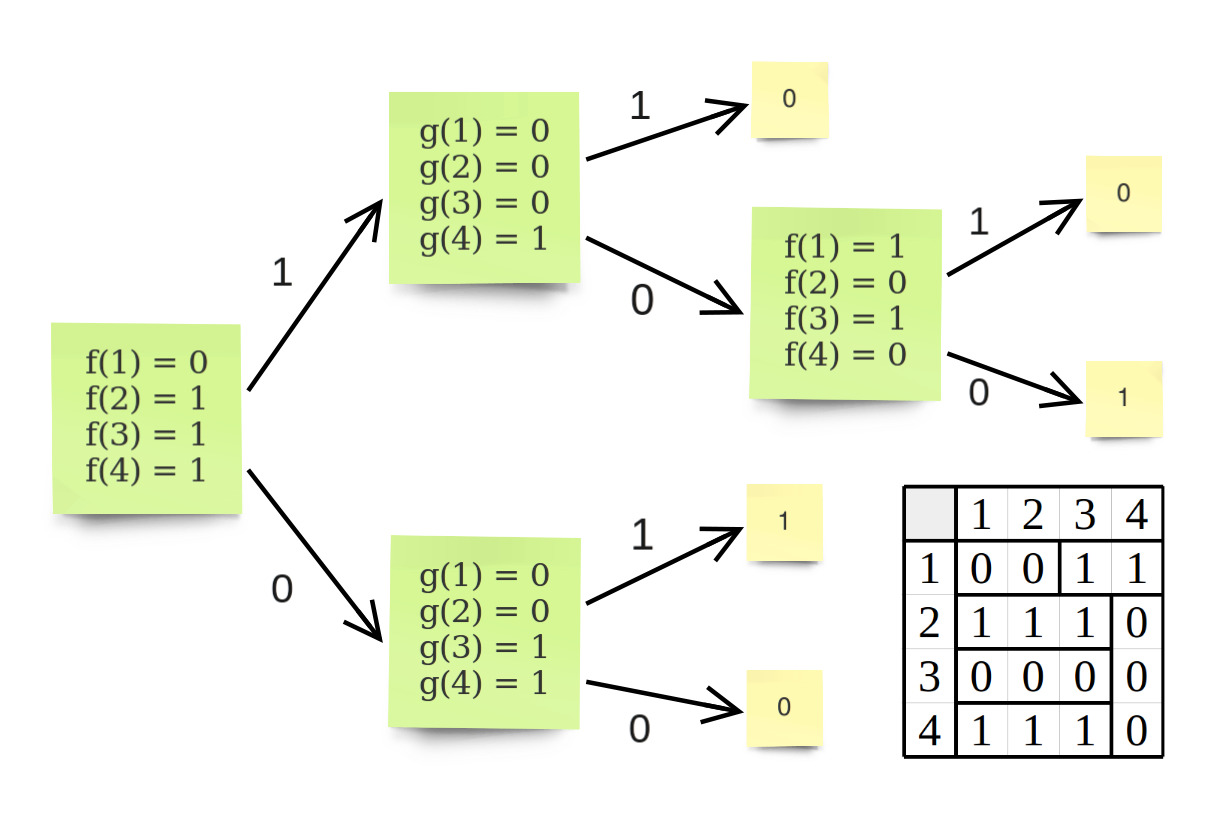
\includegraphics[width=0.8\textwidth]{images/protocol.png}
	\caption{Пример протокола и разбиения таблицы значений.}
\end{figure}

Подведем промежуточные итоги: всякий протокол с $l$ листьями (вычисляющий функцию $f$) задаёт разбиение
таблицы значений $f$ на $l$ одноцветных прямоугольных множеств. Значит, чтобы доказать, что коммуникационная 
сложность $CC(f)$ не меньше $n$, достаточно показать, что таблицу значений невозможно разбить на менее,
чем $2^n$ одноцветных прямоугольных множеств.

\subsection{Графовая интерпретация}

Давайте теперь посмотрим на другое представление множества значений функции $f$. Рассмотрим полный 
двудольный граф $G = (X, Y, E)$, ребра которого раскрашены в $|Z|$ цветов. Вершины левой доли 
соответствуют элементам множества $X$, вершины правой доли - элементам множества $Y$. Ребро 
$(x, y) \in X\times Y$ имеет цвет $z \in Z$, если $f(x, y) = z$.

Из определения комбинаторного прямоугольника видно, что в графовой интерпертации он является ничем
иным, как полным двудольным подграфом. А разбиение таблицы значений $f$ на одноцветные прямоугольные
множества -- это разбиение нашего  полного двудольного графа $G$ на одноцветные непересекающиеся биклики 
(полные двудольные подграфы). Для нашего примера графовую интерпретацию можно посмотреть на рис. 2.

\begin{figure}
	\centering
	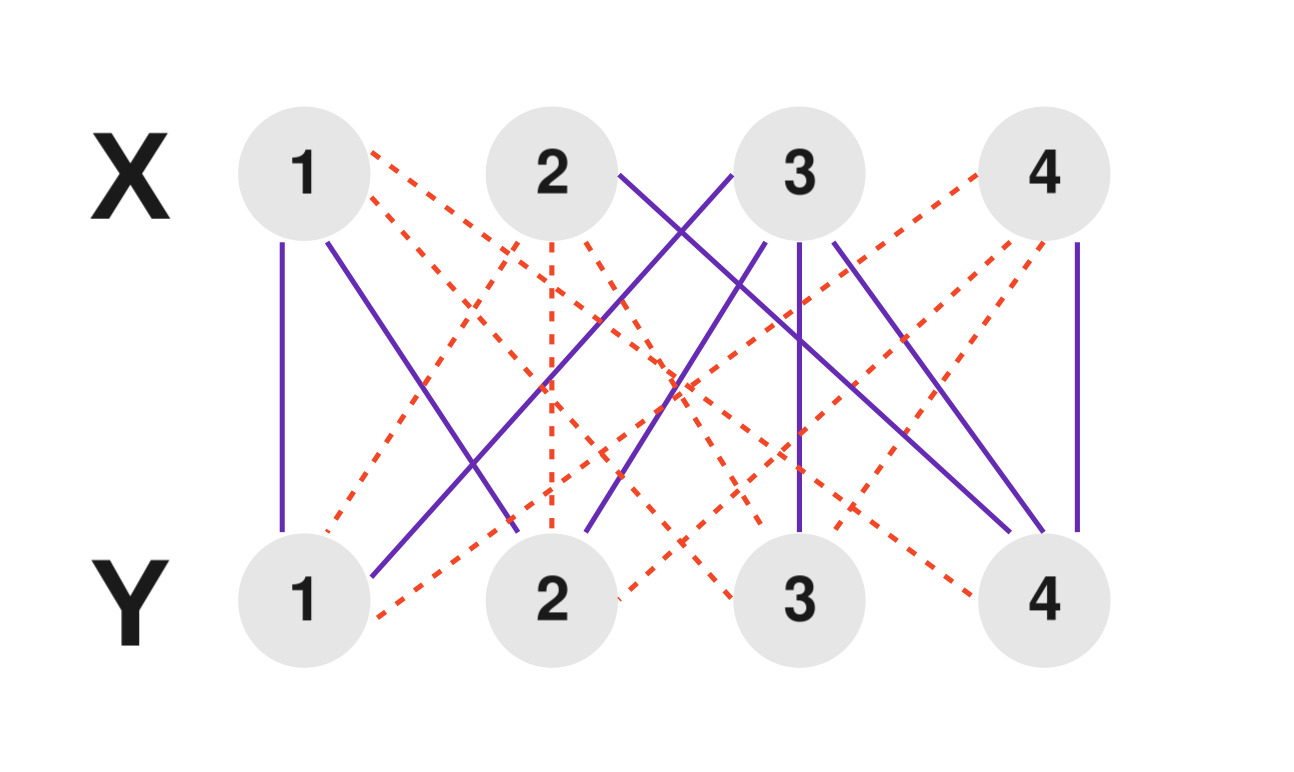
\includegraphics[width=0.6\textwidth]{images/biclique.png}
	\caption{Графовая интерпретация: синие -- 0, красные -- 1.}
\end{figure}

\begin{mdefinition}
	Бикликовым разбиением $bcp(G)$ двудольного графа $G$ будем называть наименьшее число непересекающихся
	биклик, которыми можно покрыть все ребра графа $G$.
\end{mdefinition}


\begin{mdefinition}
	Бикликовым покрытием $bcc(G)$ двудольного графа $G$ будем называть наименьшее число, возможно, 
	пересекающихся биклик, которыми можно покрыть все ребра графа $G$.
\end{mdefinition}

\begin{mclaim}
    Для произвольного двудольного графа $G$ верно $$bcp(G) \geq bcc(G)$$
\end{mclaim}

Для каждого $z \in Z$ определим двудольный граф $G_z = (X, Y, E_z)$, как граф, получающийся из $G$ 
выкидыванием всех ребер цвета, отличного от $z$. Иначе говоря $E_z = \{(x,y)\in X\times Y\ |\ f(x, y) = z \}$.

Величины $bcp(G_z)$ и $bcc(G_z)$ дают некоторую нижнюю оценку на коммуникационную сложность функции $f$, 
с которой намного удобнее работать: $$2^{CC(f)}\geq \sum\limits_{z\in Z}bcp(G_z)\geq \sum\limits_{z\in Z}bcc(G_z)$$

\begin{mremark}
    На самом деле величины $bcc(G_z)$ тесно связаны с недетерминированной коммуникационной сложностью 
    $NCC(f)$. Для произвольного множества $Z$ верно:
    \begin{itemize}[noitemsep]
        \item $2^{NCC(f)}\geq \sum\limits_{z\in Z}bcc(G_z)$,
        \item $NCC(f) \leq \lceil \log_2(\sum\limits_{z\in Z}bcc(G_z))\rceil + 1$
    \end{itemize}
    Иначе говоря, величины $bcc(G_z)$ и $NCC(f)$ по существу задают одну и ту же меру "сложности"\ функции $f$. 
    Подробнее про это можно прочитать, например, в \cite{Razborov}.
\end{mremark}

В итоге мы получили мощный иструмент для доказательства нижних оценок коммуникационной сложности. 
К сожалению, задача нахождения величины $bcc(G)$ является PSPACE-полной \cite{HermannMarkus}, а точное 
значение известно только для очень скудного класса графов (например, для "crown graphs"\ \cite{CrownGraph}), поэтому 
напрямую мы не можем использовать эту оценку. В следующей главе я рассмотрю несколько методов, 
позволяющих для произвольного двудольного графа оценивать снизу величину $bcc(G)$.

\setcounter{mclaim}{0}
\setcounter{mlemma}{0}
\setcounter{mtheorem}{0}
\addtocounter{section}{1}
\section*{Оценивание $bcc(G)$}
\addcontentsline{toc}{section}{Оценивание $bcc(G)$}

В этом разделе я опишу три различных метода оценивания бикликового покрытия:
\begin{itemize}[noitemsep]
	\item метод трудного множества ("fooling set");
	\item метод Куликова-Юкны;
	\item метод энтропийных неравенств.
\end{itemize}

Первые два метода работают для произвольных графов (необязательно двудольных), а третий применим к 
большому классу двудольных графов.

\setcounter{subsection}{0}

\subsection{Метод трудного множества}

Данный метод тесно связан с одноцветными прямоугольными множествами. Классическое определение 
трудного множества выглядит следующим образом:

\begin{mdefinition}
	Для функции $f: X\times Y \rightarrow Z$ и элемента $z\in Z$ будем называть множество 
	$S_z\subset X\times Y$ трудным (в англоязычной литературе fooling set), если верно:
	\begin{itemize}[noitemsep]
		\item для всякой пары $(x, y)\in S_z$ имеем $f(x, y) = z$;
		\item для любых двух несовпадающих пар $(x, y)\in S_z$ и $(x', y')\in S_z$ имеем 
		$f(x, y') \neq z$ или $f(x', y) \neq z$.
	\end{itemize}
\end{mdefinition}

Нас будет интересовать немного более общее определение трудного множества (графовая интерпретация):
\begin{mdefinition}
	Пусть $G = (V, E)$ произвольный неориентированный граф. Будем называть подмножество ребер 
	$S \subseteq E$ трудным, если для любых двух различных ребер $(x, y)\in S$ и $(x', y')\in S$ 
	имеем $(x, y') \notin E$ или $(x', y) \notin E$. Обозначение $fool(G)$ - размер максимального по 
	мощности трудного множества.
\end{mdefinition}

\begin{mremark}
	Классическое определение получается из графового, применением к двудольному графу $G_z = (X, Y, E_z)$, 
	который строится по функции $f: X\times Y \rightarrow Z$.
\end{mremark}

	
\begin{mtheorem}
    Для произвольного неориентированного графа $G = (V, E)$, если подмножество ребер $S \subseteq E$ 
    является трудным, то $bcc(G) \geq |S|$.
\end{mtheorem}

\begin{msolution}
    Достаточно доказать, что два ребра, лежащие одновременно в одном трудном множестве, не могут 
    попасть в одну биклику. Пусть не так, значит существуют два ребра $(x, y)\in B\cap S$ и 
    $(x', y')\in B\cap S$, где $B$ - биклика, а $S$ - трудное подмножество ребер. Но тогда ребра 
    $(x, y')$ и $(x', y)$ также принадлежат биклике $B$, а значит лежат и в нашем множестве ребер 
    $E$. Противоречие. $\blacksquare$
\end{msolution}

\subsection{Метод Куликова-Юкны}
Следующий метод был впервые описан в статье \cite{KulikovJukna}, и работает он для произвольного 
неориентированного графа.

\begin{mtheorem}
    Для произвольного неориентированного графа $G = (V, E)$ верно: $$bcc(G)\geq \left\lceil\frac{v(G)^2}{|E|}\right\rceil$$ 
    где $v(G)$ -- размер максимального паросочетания графа $G$.
\end{mtheorem}

\begin{msolution}
	Пусть $M\subseteq E$ - это максимальное паросочетание, тогда рассмотрим бикликовое покрытие, 
	на котором достигается минимум $E = B_1\cup B_2\cup \ldots \cup B_{bcc(G)}$. Определим 
	отображение $g:M\rightarrow \{1,\ \ldots,\ bcc(G)\}$, как $g(e) = min\{i\ |\ e\in B_i\}$ и пусть 
	$M_i = \{e\in M\ |\ g(e) = i\}$. Иначе говоря $M_i$ содержит только те ребра максимального 
	паросочетания $M$, которые покрываются бикликой $B_i$ впервый раз.
	
	Пусть $F_i \subseteq B_i$ биклика, индуцированная вершинами ребер из $M_i$. Пусть 
	$F = F_1\sqcup F_2\sqcup \ldots \sqcup F_{bcc(G)}$ (биклики $F_i$ не пересекаются по построению).
	
	Очевидно, что $F_i$ - биклика размера $r_i\times r_i$, где $r_i = |M_i|$. Получаем следующие 
	соотношения: $$r_1 + r_2 + \ldots + r_{bcc(G)} = |M| = v(G)$$ и 
	$$r_1^2 + r_2^2 + \ldots + r_{bcc(G)}^2 = |F|$$ Из неравенства Коши-Буняковского получаем 
	$$v(G)^2 = (r_1 + r_2 + \ldots + r_{bcc(G)})^2 \leq bcc(G)\cdot (r_1^2 + r_2^2 + \ldots + r_{bcc(G)}^2) = bcc(G)\cdot |F|$$
	А так как $F \subseteq E$, то $$v(G)^2\leq bcc(G)\cdot |F| \leq bcc(G)\cdot |E|\ \blacksquare$$

\end{msolution}

В этой же статье \cite{KulikovJukna} этот метод сравнивался с другой оценкой: пусть $bcl(G) = \max\limits_{K_{r,r}\subseteq G}\{r\}$, 
тогда
\[bcc(G) \geq \left\lceil\frac{v(G)}{bcl(G)}\right\rceil \tag{*}\]
Данная оценка очевидным образом следует из того, что любая биклика $K_{r, s}$ содержит как максимум 
$min\{r, s\}$ ребер максимального паросочетания.

Приведем примеры графов, на которых метод Куликова-Юкны работает намного лучше, чем оценка (*), и наоборот:

\begin{itemize}
    \item пусть двудольный граф $G = (L, R, E)$ состоит из совершенного паросочетания размера 
    $n = |L| = |R|$ и еще некоторого константного числа непересекающихся биклик $K_{r,r}$. 
    К тому же, пусть $r = \Theta(\sqrt{n})$, тогда $$\left\lceil\frac{v(G)^2}{|E|}\right\rceil = 
    \left\lceil\frac{n^2}{cr^2 + n}\right\rceil = \Theta(n) \gg \Theta(\sqrt{n}) = \left\lceil\frac{n}{r}\right\rceil = 
    \left\lceil\frac{v(G)}{bcl(G)}\right\rceil$$ 
    \item рассмотрим двудольный граф Леви, построенный при помощи конечной проективной плоскости порядка 
    $p\in \mathbb{P}$. В каждой доле этого графа содержится $n = p^2 + p + 1$ вершин, причем степень 
    каждой $p+1$. Этот граф не содержит $K_{2,2}$ (любые две прямые пересекаются максимум в одной точке). 
    А так как в регулярных двудольных графах обязательно найдется совершенное паросочетание, то 
    $$\left\lceil\frac{v(G)^2}{|E|}\right\rceil = \left\lceil\frac{(p^2 + p + 1)^2}{(p^2+p+1)(p+1)}\right\rceil = 
    \Theta(\sqrt{n}) \ll$$ $$\ll \Theta(n) = \left\lceil\frac{p^2 + p + 1}{1}\right\rceil = \left\lceil\frac{v(G)}{bcl(G)}\right\rceil$$
\end{itemize}




\subsection{Метод энтропийных неравенств}

Следующий метод оценивания бикликового покрытия был описан в статье \cite{EntropyInequality}, как результат 
применения энтропийного неравенства: $$H(A|B,X) + H(A|B,Y) \leq H(A|B)$$ К сожалению, это неравенство 
выполняется не для произвольного совместного распределения случайных величин $A, B, X, Y$, и соответственно 
на двудольный граф будет накладываться дополнительное условие (**).

\begin{mtheorem}
    Пусть ребра двудольного графа $G = (L, R, E)$ раскрашены следующим образом:\ \\
    (**) для произвольной биклики $C\subseteq G$ и для произвольной пары ребер $(x, y')$ и $(x', y)$ 
    из $C$, покрашеных в цвет $a$, цвет ребер $(x, y)$ и $(x', y')$ тоже $a$.\ \\
    Пусть также на ребрах этого графа задано произвольное вероятностное распределение. Определим случайные 
    величины $(X, Y, A)$ следующим образом:
    \begin{itemize}[noitemsep]
        \item $X = [$левый конец ребра$]$, 
        \item $Y = [$правый конец ребра$]$,
        \item $A = [$цвет ребра$]$.
    \end{itemize}
    Тогда выполняется неравенство: $$bcc(G) \geq 2^{\frac{1}{2}(H(A|X) + H(A|Y) - H(A))}$$
\end{mtheorem}

\begin{mexample}
    Определим двудольный граф $G_{n,k} = (L, R, E)$ следующим образом: 
    \begin{itemize}[noitemsep]
        \item $L$ и $R$ всевозможные $k$-элементные подмножества $\{1,\ 2,\ \ldots,\ n\}$,
        \item $E\subseteq L\times R$ состоит из пар непересекающихся множеств.
    \end{itemize}
    Определим цвет ребра $(x, y)\in E$, как $x\sqcup y$, и пусть на ребрах задано равномерное распределение.
    Условие (**) выполнено, потому что любые два одноцветных ребра не могут лежать в одной биклике. А так как 
    $H(A|X) = H(A|Y) = \log_2\binom{n-k}{k}$ и $H(A) = \log_2\binom{n}{2k}$, то $$bcc(G_{n,k}) \geq 
    \sqrt{\binom{n-k}{k}^2 / \binom{n}{2k}}$$
    Если $n \gg k$, то $\binom{n-k}{k}^2 / \binom{n}{2k}$ близко к $\binom{2k}{k}\approx 2^{2k}$ и мы 
    получаем нижнюю оценку $bcc(G_{n,k})\geq 2^k$.
\end{mexample}

\setcounter{mclaim}{0}
\setcounter{mlemma}{0}
\setcounter{mtheorem}{0}
\addtocounter{section}{1}
\section*{Геометрические конфигурации}
\addcontentsline{toc}{section}{Геометрические конфигурации}
В этом разделе мы приведем класс двудольных графов, построенных при помощи некоторой геометрической 
конфигурации $\Gamma$. Мы увидим, что к этим двудольным графам применимы все наши оценки, и поэтому, 
изменяя $\Gamma$, мы можем сравнить какие методы работают лучше, а какие хуже.

\setcounter{subsection}{0}
\subsection{Описание двудольного графа}
\begin{mdefinition}
    Геометрической конфигурацией $\Gamma$ (Partial Linear Space) будем называть конечное множество 
    прямых $A$ и конечное множество точек $V$ на них, что выполняются следующие две аксиомы:
    \begin{itemize}[noitemsep]
        \item Любые две точки лежат как максимум на одной прямой.
        \item На каждой прямой лежит хотя бы две точки.
    \end{itemize}
\end{mdefinition}

\begin{mdefinition}
    Геометрической конфигурацией c параметрами $(p_{\gamma}, l_{\pi})$ будем называть такую конфигурацию, которая
    состоит из $p$ точек и $l$ прямых, причем через каждую точку проходит ровно $\gamma$ прямых и на 
    каждой прямой лежит ровно $\pi$ точек. 
\end{mdefinition}

Пусть у нас имеется некоторая геометрическая конфигурация $\Gamma = (V, A)$, тогда определим двудольный 
граф $G_{n,\Gamma} = (L, R, E)$ следующим образом:
\begin{itemize}[noitemsep]
    \item $L = R = V^n$
    \item $E = \{(x, y)\in L\times R\ |\ \forall i: x_i \neq y_i$ и лежат на одной прямой из $A\}$
\end{itemize}

\subsection{Оценки для $(p_{\gamma}, l_{\pi})$}

Для геометрической конфигурации $\Gamma$ c параметрами $(p_{\gamma}, l_{\pi})$ (предполагаем, что $l \geq 3$) найдем какие 
оценки на $bcc(G_{n,\Gamma})$ дают наши методы:

\begin{itemize}[noitemsep]
    \item[--] Метод трудного множества:
    \begin{mlemma}
        Если в $\Gamma$ имеется цикл нечетной длины, то в $G_{1, \Gamma}$ можно найти трудное множество 
        размера 3.
    \end{mlemma}
    \begin{msolution}
        Рассмотрим нечетный цикл минимальной длины $\{v_1,\ v_2,\ \ldots,\ v_{2k+1}\}$, где $k \geq 1$.
        Заметим, что прямые могут проходить только через соседние точки этого цикла, иначе бы мы нашли 
        нечетный цикл меньшей длины. Тогда, если $k > 1$, то множество ребер $\{(v_1, v_2),\ (v_2, v_3),
        \ (v_3, v_4)\}$ образует трудное множество, а если $k = 1$, то $\{(v_1, v_2),\ (v_2, v_3),
        \ (v_3, v_1)\}$ образует трудное множество. $\square$
    \end{msolution}
    
    \begin{mremark}
        Если на какой-нибудь прямой лежит по крайне мере три точки $v_1, v_2, v_3$, то мы можем найти 
        трудное множество $\{(v_1, v_2),\ (v_2, v_3),\ (v_3, v_1)\}$ размера 3.
    \end{mremark}

     Если  в $\Gamma$ нет нечетных циклов и на каждой прямой лежит ровно 2 точки, то мы получаем 
     геометрическую конфигурацию, аналогичную двудольному графу. Если этот двудольный граф полный, 
     то наибольшее трудное множество имеет размер 2, а если неполный, то рассмотрим два случая:
     \begin{itemize}
         \item[1)] Если $\gamma = 1$, то $\Gamma$ является паросочетанием, а значит все ребра графа 
         $G_{1,\Gamma}$ образуют трудное множество (ребер ровно $l \geq 3$).
         \item[2)] Если $\gamma \geq 2$ и нет прямой проходящей через точки $v_1$ и $v_2$ из разных долей, 
         то существуют точки $v_3, v_4, v_5, v_6$ такие, что прямые проходят через пары точек $(v_1, v_4), 
         (v_2, v_3)$ и $(v_2, v_5)$. Но тогда множество ребер $\{(v_1, v_4), (v_3, v_2), (v_2, v_5)\}$ 
         образуют трудное множество размера 3.
     \end{itemize}
     Иначе говоря, мы показали, что если $\Gamma$ аналог не полного двудольного графа, то мы можем 
     найти трудное множество размера 3. 

     
     \begin{mlemma}
         Если в $G_{1, \Gamma}$ существует трудное множество размера $k$, то в $G_{n, \Gamma}$ 
         существует трудное множество размера $k^n$
     \end{mlemma}
     \begin{msolution}
        Докажем вначале, что если в графе $G_1$ имеется трудное множество размера $n_1$, а в графе 
        $G_2$ -- трудное множество размера $n_2$, тогда в $G_1 \otimes G_2$ можно найти трудное 
        множество размера $n_1\cdot n_2$ (где $\otimes$ - произведение Кронекера). Пусть $\{v_{i,j}\}$ 
        трудное множество в графе $G_1$, тогда в каждой подматрице $v_{i, j}\cdot G_2$ матрицы 
        графа $G_1 \otimes G_2$ рассмотрим клетки, соответствующие трудному множеству графа $G_2$. 
        Всего мы получили $n_1\cdot n_2$ клеток, образующих трудное множество графа $G_1 \otimes G_2$ 
        по построению.
        
        Вернемся к доказательству леммы. Так как матрица графа $G_{n, \Gamma}$ есть не что иное, как 
        Кронекерово произведение $n$ матриц графа $G_{1, \Gamma}$, то мы можем найти трудное множество 
        размера $k^n$. $\square$
     \end{msolution}
     
     В итоге мы получили, что если $\Gamma$ является аналогом полного двудольного графа, то 
     $$bcc(G_{n, \Gamma}) \geq 2^n$$ иначе $$bcc(G_{n, \Gamma}) \geq 3^n$$
     
     \item[--] Метод Куликова-Юкны:
     
     Так как $\Gamma$ имеет параметры $(p_{\gamma}, l_{\pi})$, то каждая вершина графа $G_{1,\Gamma}$ 
     соединена с $\gamma\cdot (\pi - 1)$ другими, а значит всего ребер $\gamma\cdot (\pi - 1)\cdot p$. Тогда в графе 
     $G_{n, \Gamma}$ всего ребер $\gamma^n\cdot (\pi - 1)^n\cdot p^n$. Так как у нас однородный двудольный граф, 
     то имеется совершенное паросочетание, а значит $v(G_{n, \Gamma}) = p^n$. В итоге получаем оченку:
     $$bcc(G_{n,\Gamma}) \geq \frac{p^{2n}}{\gamma^n\cdot (\pi - 1)^n\cdot p^n} = \left(\frac{p}{\gamma\cdot (\pi -1)}\right)^n$$
     
     \item[--] Метод энтропийных неравенств:
     
     Определим раскраску ребер нашего графа $G_{n,\Gamma} = (L, R, E)$: сопоставим каждой прямой из
     конфигурации $\Gamma$ свой цвет, тогда цвет ребра $(x, y)\in E$ равен $n$-мерному вектору цветов 
     прямых, проходящих через $x_i$ и  $y_i$.
     
     Проверим свойство (**): пусть $(x, y')$ и $(x', y)$ одного цвета и лежат в одной биклике $C$, значит 
     для любого $i$ точки $x_i,\ y'_i,\ x'_i,\ y_i$ лежат на одной прямой (некоторые точки могут совпадать), 
     но тогда очевидно, что ребро $(x, y)$ такого же цвета. 
     
     Пусть на ребрах графа задано равномерное распределение, тогда $H(A) = \log_2l^n = n\cdot\log_2l$ и 
     $H(A|X)=H(A|Y) = \log_2\gamma^n = n\cdot\log_2\gamma$. В итоге получаем оценку: $$bcc(G_{n, \Gamma}) \geq 
     2^{n\cdot\log_2\gamma - \frac{n}{2}\cdot\log_2l} = \left(\frac{\gamma}{\sqrt{l}}\right)^n$$
     
\end{itemize}

\subsection{Сравнение методов оценивания}

Рассмотрим какие оценки получаются на известных геометрических конфигурациях. Симметричные конфигурации ($p = l$ и 
$\gamma = \pi$) будем обозначать сокращенно $(p_{\gamma})$.
\newpage

\begin{table}[h]
	\begin{tabular}{|>\centering m{4cm}|c|c|c|c|}
		\hline
		Название & FS & KJ & EI & Результат \\ \hline
		Треугольник\newline$\left(3_2\right)$ & $\geq 3^n$ & $\left(\frac{3}{2}\right)^n$ & $\left(\frac{2}{\sqrt{3}}\right)^n$ & $FS > KJ > EI$ \\ \hline
		Полный четырехсторонник\newline$\left(4_3,\ 6_2\right)$ & $\geq 3^n$ & $\left(\frac{4}{3}\right)^n$ & $\left(\frac{3}{\sqrt{6}}\right)^n$ & $FS > KJ > EI$ \\ \hline
		$K_m$ при $m>4$\newline$\left(m_{m-1},\ \binom{m}{2}_2\right)$ & $\geq 3^n$ & $\left(\frac{m}{m-1}\right)^n$ & $\left(\sqrt{\frac{2(m-1)}{m}}\right)^n$ & $FS > EI > KJ$ \\ \hline
		$K_{m, m}$ при $m>0$\newline$\left(2m_m,\ m^2_2\right)$ & $\geq 2^n$ & $2^n$ & $1^n$ & $FS = KJ > EI$ \\ \hline
		Плоскость Фано\newline$\left(7_3\right)$  & $\geq 3^n$ & $\left(\frac{7}{6}\right)^n$ & $\left(\frac{3}{\sqrt{7}}\right)^n$ & $FS > KJ > EI$ \\ \hline
		Конфигурация Мёбиуса-Кантора\newline$\left(8_3\right)$  & $\geq 3^n$ & $\left(\frac{4}{3}\right)^n$ & $\left(\frac{3}{\sqrt{8}}\right)^n$ & $FS > KJ > EI$ \\ \hline
		Конфигурация Дезарга $\left(10_3\right)$  & $\geq 3^n$ & $\left(\frac{5}{3}\right)^n$ & $\left(\frac{3}{\sqrt{10}}\right)^n$ & $FS > KJ > EI$ \\ \hline
		Конфигурация Гессе $\left(9_4,\ 12_3\right)$  & $\geq 3^n$ & $\left(\frac{9}{8}\right)^n$ & $\left(\frac{2}{\sqrt{3}}\right)^n$ & $FS > EI > KJ$ \\ \hline
		Конфигурация Шлефли $\left(12_5,\ 30_2\right)$  & $\geq 3^n$ & $\left(\frac{12}{5}\right)^n$ & $\left(\frac{5}{\sqrt{30}}\right)^n$ & $FS > KJ > EI$ \\ \hline
		Проективная плоскость $\left((m^2 + m + 1)_{m+1}\right)$  & $\geq 3^n$ & $\left(\frac{m^2+m+1}{m(m+1)}\right)^n$ & $\left(\frac{m+1}{\sqrt{m^2 + m + 1}}\right)^n$ & $FS > EI > KJ$ \\ \hline
		Конфигурация Кокса $\left((2^{m-1})_m\right)$  & $\geq 3^n$ & $\left(\frac{2^{m-1}}{m(m-1)}\right)^n$ & $\left(\frac{m}{\sqrt{2^{m-1}}}\right)^n$ & $FS > KJ > EI$ \\
		\hline
	\end{tabular}
\end{table}

Из таблицы видно, что метод трудного множества всегда работает лучше, чем остальные. 
Почти во всех примерах мы нашли трудное множество размера $3^n$, но максимальное трудное множество 
может иметь очень большой размер. Оценки $3^n$ не достаточно, чтобы доказать, что на геометрических конфигурациях 
метод трудного множества всегда работает лучше, чем оценка Куликова-Юкны, но зато достаточно для 
метода энтропийных неравенств:

\begin{mclaim}
    Для произвольной геометрической конфигурации $(p_{\gamma}, l_{\pi})$ оценка, получаемая по методу 
    трудного множества, превосходит оценку метода энтропийных неравенств. Иначе говоря 
    $$2 \geq \frac{\gamma}{\sqrt{l}}$$
\end{mclaim}

\begin{msolution}
	Условия 
	\begin{equation*}
	    \begin{cases}
			p\cdot \gamma = l\cdot \pi, \\
			p \geq \gamma\cdot (\pi - 1) + 1.
		\end{cases}
	\end{equation*}
	должны обязательно выполняться для того, чтобы геометрическая конфигурация была корректно определена.
	
	Используя эти ограничения, получаем $$\frac{\gamma^2}{l} = \frac{\pi\cdot\gamma}{p} \leq \frac{p + 
	\gamma - 1}{p} = 1 + \frac{\gamma - 1}{p} < 4$$
	
	Что и требовалось доказать. $\square$
\end{msolution}

Теперь давайте сравним метод Куликова-Юкны и метод энтропийных неравенств. Рассмотрим два случая:
\begin{itemize}[noitemsep]
    \item Пусть выполняется условие $l \geq \gamma^2$, тогда $$\gamma^2 \cdot (\pi - 1) \leq l \cdot (\pi - 1) 
    < p\cdot\gamma \leq p\cdot\sqrt{l}$$ То есть получаем, что $KJ > EI$.
    \item Пусть теперь верно $l \leq \gamma^2$, тогда $$\gamma^2\cdot (\pi - 1) \geq l\cdot(\pi - 1) = 
    p\cdot\gamma - l \geq p\cdot\sqrt{l} - l$$ Поделив обе части на $\sqrt{l}\cdot\gamma\cdot(\pi -1)$, 
    получаем $$\frac{\gamma}{\sqrt{l}} \geq \frac{p}{\gamma\cdot(\pi - 1)} - \frac{\sqrt{l}}{\gamma\cdot(\pi-1)}$$
	В итоге получаем, что с небольшой погрешностью $EI \gtrsim KJ$
\end{itemize}

\setcounter{mclaim}{0}
\setcounter{mlemma}{0}
\setcounter{mtheorem}{0}
\addtocounter{section}{1}
\section*{Теорема Турана и граф четырехсторонников}
\addcontentsline{toc}{section}{Теорема Турана и граф четырехсторонников}
В этом разделе мы докажем, что метод трудного множества всегда дает оценку лучше, чем метод Куликова-Юкны. 
Также мы сведем задачу нахождения $bcc(G)$ к задаче поиска хроматического числа графа, 
что позволит нам получить переформулированный метод трудного множества и обобщение оценки (*).  

\setcounter{subsection}{0}
\subsection{Теорема Турана и ее следствие}
Как уже видно из названия, для дальнейших изысканий нам потребуется классическая теорема Турана:
\begin{mtheorem}\emph{\textbf{(Туран)}}
    Пусть дан неориентированный граф $G = (V, E)$, где $|V| = n$ и число независимости равно $\alpha$. 
    Тогда в графе выполняется следующая оценка $$|E| \geq n\cdot\left[\frac{n}{\alpha}\right] - 
    \alpha\cdot\frac{\left[\frac{n}{\alpha}\right]\cdot\left(\left[\frac{n}{\alpha}\right] + 1\right)}{2}$$
\end{mtheorem}

Доказательство этой теоремы можно найти в книге $\cite{OreOustin}$. Используя эту теорему, мы можем доказать следующее:
\begin{mtheorem}
    Пусть имеется неориентированный граф $G = (V, E)$, тогда среди ребер максимального паросочетания можно 
    найти трудное множество размера $$\left\lceil\frac{v(G)^2}{|E|}\right\rceil$$
\end{mtheorem}

\begin{msolution}
    Давайте вместо графа $G = (V, E)$ рассмотрим граф $\widehat{G} = (\widehat{V}, \widehat{E})$, 
    в котором останутся только вершины из максимального паросочетания. Так как $|E| \geq |\widehat{E}|$, то
    достаточно найти трудное множество размера $$\left\lceil\frac{v(G)^2}{|\widehat{E}|}\right\rceil$$
    Пусть $(v_1, v'_1),\ (v_2, v'_2),\ \ldots,\ (v_m, v'_m)$ -- ребра максимального паросочетания. 
    Построим граф $\widetilde{G} = (\widetilde{V}, \widetilde{E})$ такой, что вершин в нем ровно $m$. 
    Обозначим вершины $\{\widetilde{v}_1,\ \widetilde{v}_2,\ \ldots,\ \widetilde{v}_m\}$, причем 
    $\widetilde{v}_i \leftrightarrow (v_i, v'_i)$. Определим множество ребер $\widetilde{E}$ следующим образом 
    $$(\widetilde{v}_i, \widetilde{v}_j)\in \widetilde{E} \hbox{ если } (v_i, v'_i)\notin \widehat{E} 
    \hbox{ или } (v_j, v'_j)\notin \widehat{E}$$ Очевидно, что трудное множество на ребрах максимального 
    паросочетания соответствует клике в $\widetilde{G}$ такого же размера. Пусть число независимости 
    дополнения графа $\widetilde{G}$ равно $\alpha$, тогда мы можем предъявить трудное множество размера 
    $\alpha$. Используя теорему Турана для дополнения графа $\widetilde{G}$, получаем $$|\overline{\widetilde{E}}| \geq 
    m\cdot\left[\frac{m}{\alpha}\right] - \alpha\cdot\frac{\left[\frac{m}{\alpha}\right]\cdot\left(
    \left[\frac{m}{\alpha}\right] + 1\right)}{2} = $$ Пусть $m = k\cdot \alpha + r$, где $r < \alpha$ 
    $$ = (k\cdot\alpha + r)\cdot k - \alpha\cdot\frac{k\cdot(k+1)}{2} = \frac{\alpha\cdot k^2}{2} + 
    r\cdot k - \frac{\alpha\cdot k}{2}$$ Так как каждое ребро из дополнения графа $\widetilde{G}$ порождает 
    два ребра в $\widehat{G}$, а также еще имеется $m$ ребер самого паросочетания, то получаем 
    $$|\widehat{E}| \geq m + 2\cdot\left(\frac{\alpha\cdot k^2}{2} + r\cdot k - \frac{\alpha\cdot k}{2}\right) = $$
    $$ = \alpha\cdot k^2 + 2r\cdot k + r \geq \alpha\cdot k^2 + 2r\cdot k + \left\lceil\frac{r^2}{\alpha}\right\rceil = 
    \left\lceil\frac{m^2}{\alpha}\right\rceil$$ В итоге получили, что $$|\widehat{E}|\geq 
    \left\lceil\frac{m^2}{\alpha}\right\rceil \Longleftrightarrow \alpha \geq \left\lceil\frac{m^2}{|\widehat{E}|}\right\rceil = 
    \left\lceil\frac{v(G)^2}{|\widehat{E}|}\right\rceil \blacksquare$$
\end{msolution}

Эта теорема говорит нам о том, что на любом неориентированном графе точная оценка по методу трудного множества лучше, 
чем оценка Куликова-Юкны.

\subsection{Граф четырехсторонников}
При доказательстве предыдущей теоремы мы использовали некоторый модифицированный граф $\widetilde{G} = 
(\widetilde{V}, \widetilde{E})$. По аналогии можно рассмотреть более общую конструкцию, которую мы 
будем называть графом четырехсторонников. 
\begin{mdefinition}
    Пусть имеется двудольный неориентированный граф $G = (L, R, E)$. Определим граф четырехсторонников 
    $\widetilde{G} = (\widetilde{V}, \widetilde{E})$ следующим образом:
    \begin{itemize}[noitemsep]
        \item $e_{i,j}\in E \leftrightarrow v_{i,j}\in \widetilde{V}$, значит $|E| = |\widetilde{V}|$.
        \item $(v_{i,j}, v_{k, l}) \in \widetilde{E}$ тогда и только тогда, когда $v_{i,l}\notin \widetilde{E}$ 
        или $v_{k,j}\notin\widetilde{E}$
    \end{itemize}
\end{mdefinition}

Введем также понятия хроматического, кликового и антикликового чисел:
\begin{mdefinition}

    Хроматическое число графа $G$ -- минимальное число $k$ такое, что множество вершин графа можно 
    покрасить в $k$ цветов, причем любое ребро графа соединяет разноцветные вершины. Обозначение $\chi(G)$.
\end{mdefinition}
\begin{mdefinition} 
    Кликовое число графа $G$ -- максимальное число $k$ такое, что в нашем графе содержится полный 
    граф на $k$ вершинах ($k$-клика). Обозначение $w(G)$.
\end{mdefinition}
\begin{mdefinition} 
    Антикликовое число графа $G$ -- максимальное число $k$ такое, что в графе дополнения содержится 
    полный граф на $k$ вершинах ($k$-антиклика). Обозначение $\alpha(G)$.
\end{mdefinition}


Используя конструкцию графа четырехсторонников, мы можем сформулировать следующую теорему:
\begin{mtheorem}
    Для любого двудольного графа $G = (L, R, E)$ верно:
    \begin{itemize}[noitemsep]
        \item[1)] $fool(G) = w(\widetilde{G})$
        \item[2)] $\max\limits_{K_{r,s}\subseteq G}\{r\cdot s\} = \alpha(\widetilde{G})$
        \item[3)] $bcc(G) = \chi(\widetilde{G})$
    \end{itemize}
\end{mtheorem}



\begin{msolution}
    Так как каждому трудному множеству размера $k$ в $G$ соответствует $k$-клика в $\widetilde{G}$ и 
    наоборот, то $fool(G) = w(\widetilde{G})$.
    
    Очевидно, что биклике $K_{r,s}$ в $G$, соответствует антиклика размера $r\cdot s$ в $\widetilde{G}$. 
    Обратно, если $(v_{i,j}, v_{k,l}) \notin \widetilde{E}$, то вершины $v_{i, l}$ и $v_{k, j}$ 
    определены, и между ними нет ребра. И следовательно, если рассмотреть какую-нибудь антиклику в 
    $\widetilde{G}$, то ее можно расширить до "прямоугольной"\  антиклики, которой будет соответствовать 
    биклика в $G$.
    
    Последняя часть теоремы сразу следует из того, что все вершины антиклики мы можем красить в один цвет. Имея 
    произвольное покрытие $bcc(G)$, мы получаем покрытие вершин графа $\widetilde{G}$ антикликами. 
    Пусть каждой биклике из $bcc(G)$ сопоставлен свой цвет. Красим вершину в тот цвет, который соответствует 
    покрывающей ее биклике (если таких биклик несколько, то в любой из них). В итоге получаем правильную 
    раскраску графа в $bcc(G)$ цветов. Обратно, правильная покраска графа $\widetilde{G}$ порождает 
    покрытие антикликами, которые мы расширяем до "прямоугольных". А так как эти антиклики
    соответствуют бикликам в $G$, то мы получили покрытие бикликами (возможно пересекающимися) 
    размера $\chi(\widetilde{G})$. $\blacksquare$
\end{msolution}

Эта теорема позволяет нам  переформулировать известные оценки для хроматического числа нового графа 
$\widetilde G$ в виде оценок для величины минимального бикликового покрытия исходного графа $G$
$$ \chi(\widetilde{G}) \geq w(\widetilde{G}) \Longleftrightarrow bcc(G) \geq fool(G)$$
и $$\chi(\widetilde{G}) \geq \left\lceil\max\limits_{U\subseteq \widetilde{V}}\frac{|U|}{\alpha(\widetilde{G}(U))}\right\rceil 
\Longleftrightarrow bcc(G) \geq \left\lceil\max\limits_{\mathcal{E}\subseteq E}\frac{|\mathcal{E}|}
{\max\limits_{K_{r,s}\subseteq G(\mathcal{E})}|K_{r,s}\cap\mathcal{E}|}\right\rceil$$ где $G(\mathcal{E})$ наименьший подграф $G$, 
содержащий все ребра $\mathcal{E}$. 

Если в качестве $\mathcal{E}$ рассмотреть максимальное паросочетание, тогда $\max\limits_{K_{r,s}\subseteq 
G(\mathcal{E})}|K_{r,s}\cap\mathcal{E}| = \max\limits_{K_{r,r}\subseteq G(\mathcal{E})}|K_{r,r}\cap\mathcal{E}| = 
\max\limits_{K_{r,r}\subseteq G(\mathcal{E})}\{r\} \leq \max\limits_{K_{r,r}\subseteq G}\{r\} = bcl(G)$. В итоге 
получаем оценку, которую мы уже раньше встречали: $$bcc(G) \geq \left\lceil\max\limits_{\mathcal{E}\subseteq E}\frac{|\mathcal{E}|}
{\max\limits_{K_{r,s}\subseteq G(\mathcal{E})}|K_{r,s}\cap\mathcal{E}|}\right\rceil  \geq \left\lceil\frac{v(G)}{bcl(G)}\right\rceil$$

Если же в качестве $\mathcal{E}$ взять вообще все ребра, то $$bcc(G) \geq \left\lceil\max\limits_{\mathcal{E}\subseteq E}\frac{|\mathcal{E}|}
{\max\limits_{K_{r,s}\subseteq G(\mathcal{E})}|K_{r,s}\cap\mathcal{E}|}\right\rceil \geq \left\lceil\frac{|E|}
{\max\limits_{K_{r,s}\subseteq G}\{r\cdot s\}}\right\rceil$$

\setcounter{mclaim}{0}
\setcounter{mlemma}{0}
\setcounter{mtheorem}{0}
\addtocounter{section}{1}
\section*{Случайные графы}
\addcontentsline{toc}{section}{Случайные графы}
В этом разделе мы докажем существование двудольных графов, у которых оценки по методу трудного множества и 
по методу Куликова-Юкны очень сильно отличаются. Доказывать этот факт мы будем вероятностным методом, 
используя модель Эрдеша-Реньи.

\setcounter{subsection}{0}
\subsection{Случайные двудольные графы Эрдеша-Реньи}

Пусть у нас имеются два $n$-элементных множества $L$ и $R$, элементы которого будем называть вершинами 
левой и правой долей графа. Понятно, что случайным будет множество ребер графа. Мы рассматриваем 
неориентированные графы без петель и кратных рёбер, поэтому потенциальных ребер не больше, чем $n^2$ штук. 
Будем соединять любые две вершины $i \in L$ и $j \in R$ ребром с некоторой вероятностью $p\in [0, 1]$ 
независимо от всех остальных $n^2 - 1$ пар вершин. Иными словами, ребра появляются в соответствии со 
стандартной схемой Бернулли, в которой $n^2$ испытаний и "вероятность успеха"\ $p$. Обозначим через $E$
случайное множество ребер, которое возникает в результате реализации такой схемы. Положим $G = (L, R, E)$. 
Это и есть случайный двудольный граф в модели Эрдеша – Реньи. 

Если записывать приведенное только что определение в формате аксиоматики Колмогорова, то мы имеем 
вероятностное пространство $$G(n, p) = (\Omega_n, \mathcal{F}_n, P_{n,p})$$ в котором 
$$\Omega_n = \{G = (L, R, E)\},\ \mathcal{F}_n = 2^{\Omega_n},\ P_{n,p}(G) = p^{|E|}\cdot(1-p)^{n^2 -|E|}$$

Если нам хочется найти вероятность, с которой двудольный граф на $2n$ вершинах обладает данным свойством $A$, 
то мы просто берем множество $\mathcal{A} \in \mathcal{F}_n$, состоящее из всех графов, для которых 
выполнено свойство $A$, и вычисляем $$P_{n,p}(\mathcal{A}) = \sum\limits_{G\in\mathcal{A}}P_{n,p}(G)$$

Далее будем рассматривать не фиксированное $p$, а некоторую функцию $p(n)$, заключенную между нулем и единицей. 
Скажем, наконец, что свойство выполнено почти всегда, если его вероятность стремится к единице при $n \rightarrow \infty$.

\subsection{Неравенство Хефдинга}

Пусть $\xi_1,\ \xi_2,\ \dots,\ \xi_n$ -- последовательность независимых случайных величин таких, что 
для любого $i = 1,\ 2,\ \ldots,\ n$ верно $\xi_i \in [a_i, b_i]$ с вероятностью 1 для некоторых 
$a_i, b_i \in \mathbb{R}$. Введем обозначение $S_n = \sum\limits_{i = 1}^n\xi_i$. Мы хотим изучать 
отклонение случайной величины $S_n$ от ее среднего значения $\mathbb{E}[S_n]$. Иначе говоря, получить неравенство 
концентрации для $\xi = S_n - \mathbb{E}[S_n]$. Воспользовавшись для этого неравенством Чернова получим, что 
для любого $\lambda > 0$ верно $$P\{S_n - \mathbb{E}[S_n] \geq \varepsilon\} = P\{e^{\lambda(S_n - 
\mathbb{E}[S_n])} \geq e^{\lambda\varepsilon}\} \leq \frac{\mathbb{E}[e^{\lambda(S_n - \mathbb{E}[S_n])}]}{e^{\lambda\varepsilon}} = $$
$$ = \frac{\mathbb{E}[e^{\lambda\sum\limits_{i=1}^n(\xi_i - \mathbb{E}[\xi_i])}]}{e^{\lambda\varepsilon}} = 
\frac{\mathbb{E}[\prod\limits_{i=1}^ne^{\lambda(\xi_i - \mathbb{E}[\xi_i])}]}{e^{\lambda\varepsilon}} = 
\frac{\prod\limits_{i=1}^n\mathbb{E}[e^{\lambda(\xi_i - \mathbb{E}[\xi_i])}]}{e^{\lambda\varepsilon}}$$

Нам остается построить верхние оценки для производящих функций $\varphi_{\xi_i}(\lambda)$. Следующий 
результат дает нам такие оценки в тех случаях, когда случайные величины $\xi_i$ принимают значения 
из ограниченных интервалов.

\begin{mlemma}\emph{\textbf{(Хефдинг)}}
    Для произвольной случайной величины $\xi$ такой, что $\mathbb{E}[\xi] = 0$ и $\xi \in [a, b]$ с вероятностью 1 
    для любого $\lambda > 0$ справедливо $$\mathbb{E}[e^{\lambda\xi}] \leq e^{\frac{\lambda^2(b-a)^2}{8}}$$
\end{mlemma}

Доказательство основано на выпуклости экспоненты.

Применив эту лемму к нашей цепочке неравенств для случайных величин $\xi_i - \mathbb{E}[\xi_i]$, которые
почти наверное лежат в интервалах $[a_i - \mathbb{E}[\xi_i], b_i - \mathbb{E}[\xi_i]]$, мы получаем 
$$P\{S_n - \mathbb{E}[S_n] \geq \varepsilon\} \leq \frac{\prod\limits_{i=1}^n\mathbb{E}[e^{\lambda(\xi_i - \mathbb{E}[\xi_i])}]}{e^{\lambda\varepsilon}} \leq 
 \frac{\prod\limits_{i=1}^ne^{\lambda^2(b_i-a_i)^2/8}}{e^{\lambda\varepsilon}} = \frac{e^{\lambda^2\sum\limits_{i=1}^n(b_i-a_i)^2/8}}{e^{\lambda\varepsilon}}$$

Остается минимизировать правую часть по $\lambda \geq 0$. Выбирая $$\lambda = \frac{4\varepsilon}{\sum\limits_{i=1}^n(b_i-a_i)^2}$$ 
мы получаем следующий результат 
\begin{mtheorem}\emph{\textbf{(Неравенство Хефдинга)}}
    Пусть $\xi_1,\ \xi_2,\ \dots,\ \xi_n$ -- последовательность независимых случайных величин, таких что 
для любого $i = 1,\ 2,\ \ldots,\ n$ верно $\xi_i \in [a_i, b_i]$ с вероятностью 1 для некоторых 
$a_i, b_i \in \mathbb{R}$. Тогда для любого $\varepsilon > 0$ верно $$P\{S_n - \mathbb{E}[S_n]\geq 
\varepsilon\} \leq exp\left(\frac{-2\varepsilon^2}{\sum\limits_{i=1}^n(b_i - a_i)^2}\right)$$
\end{mtheorem}

Аналогичное неравенство верно для $P\{\mathbb{E}[S_n] - S_n\geq \varepsilon\}$, поскольку условия теоремы 
инвариантны относительно замены знака слагаемых. Применив дважды неравенство Хефдинга, мы получаем 
$$P\{|S_n - \mathbb{E}[S_n]|\geq \varepsilon\} \leq P\{S_n - \mathbb{E}[S_n]\geq \varepsilon\} + 
P\{\mathbb{E}[S_n] - S_n\geq \varepsilon\} \leq $$ $$\leq 2\cdot exp\left(\frac{-2\varepsilon^2}{\sum\limits_{i=1}^n(b_i - a_i)^2}\right)$$

Воспользуемся этим неравенством для того, чтобы изучить отклонение числа ребер в случайном двудольном 
графе Эрдеша-Реньи. Определим индикаторные случайные величины $X_{i, j} = I\{e_{i,j}\in E\}$. Так как случайная 
величина $|E| = \sum\limits_{i,j}X_{i,j}$, то получаем $$\mathbb{E}[|E|] = \sum\limits_{i,j}\mathbb{E}[X_{i,j}] = 
\sum\limits_{i,j}P\{e_{i,j}\in E\} = n^2\cdot p$$

Наконец, воспользуемся неравенством Хефдинга для $\varepsilon = n^{1+\delta}$ $$ P\{||E| - \mathbb{E}[|E|]| \geq
n^{1+\delta}\} \leq 2\cdot e^{-\frac{2n^{2+2\delta}}{n^2}} = 2\cdot e^{-2n^{2\delta}} \xrightarrow[n \to \infty]{} 0 $$ 
В итоге мы получили, что почти наверное число ребер в графе не сильно отличается от его матожидания: 
$$n^2\cdot p - n^{1+\delta} \leq |E| \leq n^2\cdot p + n^{1+\delta}$$.


\subsection{Размер максимального паросочетания}

Для изучения отклонения величины максимального паросочетания нам потребуется теорема Холла.
\begin{mtheorem}\emph{\textbf{(Холл)}}
    Пусть имеется неориентированный двудольный граф $G = (L, R, E)$. Для произвольного $A \subseteq L$ 
    определим множество соседей  $$N(A) = \{y\in R\ |\ (x, y) \in E,\ x\in A\}$$ В двудольном графе существует 
    совершенное паросочетание тогда и только тогда, когда для любого $A \subseteq L$ выполнено $|A| \leq |N(A)|$.
\end{mtheorem}

Пусть имеется двудольный граф Эрдеша-Реньи $G = (L, R, E)$, где $|L| = |R| = n$. Множество 
$S \subseteq L$ не удовлетворяет условию теоремы Холла, если существует множество $T \subseteq R$ 
такое, что $|S| + |T| = n + 1$  и $N(S)\cap T = \varnothing$ (нет ребер между множествами $S$ и $T$).

Очевидно, что $$P\{N(S)\cap T = \varnothing\} = (1-p)^{|S|\cdot|T|}$$ тогда $$P\{\hbox{нет совершенного паросочетания}\} \leq 
\sum\limits_{S}\sum\limits_{T}(1-p)^{|S|\cdot|T|} = $$ $$ = \sum\limits_{k=1}^n\binom{n}{k}\binom{n}{n-k+1}(1-p)^{k(n-k+1)} \leq 
\sum\limits_{k=1}^{(n+1)/2}\binom{n}{k}\binom{n}{k-1}(1-p)^{kn/2} \leq $$ $$ \leq \sum\limits_{k=1}^{(n+1)/2}n^{2k}(1-p)^{kn/2}$$

Если предположить, что $p = p(n) = n^{-\alpha}$ при $\alpha < 1$, то получаем $$P\{\hbox{нет совершенного паросочетания}\} \leq 
\sum\limits_{k=1}^{(n+1)/2}n^{2k}(1-p)^{kn/2} = $$ $$ = \sum\limits_{k=1}^{(n+1)/2}n^{2k}e^{-\frac{kn}{2}\cdot n^{-\alpha} + O(n^{1 - 2\alpha})\cdot k} = 
\sum\limits_{k=1}^{(n+1)/2}\left(n^2e^{-\frac{1}{2}n^{1-\alpha} + O(n^{1-2\alpha})}\right)^k \xrightarrow[n \to \infty]{} 0$$

Последнее утверждение верно потому, что c некоторого момента величина стоящая под степенью будет меньше 1, 
а значит первое слагаемое будет больше всех остальных $$\sum\limits_{k=1}^{(n+1)/2}\left(n^2e^{-\frac{1}{2}n^{1-\alpha} + O(n^{1-2\alpha})}\right)^k \leq 
\frac{n+1}{2}\left(n^2e^{-\frac{1}{2}n^{1-\alpha} + O(n^{1-2\alpha})}\right) \xrightarrow[n \to \infty]{} 0$$ 

В итоге мы получили, что почти наверное (при $n \rightarrow \infty$) в нашем графе будет совершенное паросочетание.

\subsection{Трудное множество и оценка Куликова-Юкны на случайных графах}

Если предположить, что $p = p(n) = n^{-\alpha}$ ($0 < \alpha < 1$), то можно доказать следующее утверждение:
\begin{mclaim}
	Для произвольного $\delta$ такого, что $0 < \delta < 1 - \alpha$  верно:
    $$n^{\alpha} - O(n^{2\alpha + \delta - 1}) \leq \frac{v(G)^2}{|E|} \leq n^{\alpha} + O(n^{2\alpha + \delta - 1})$$
\end{mclaim}

\begin{msolution}
   Рассмотрим вероятность 
   $$P\left\{\frac{n^2}{n^{2-\alpha} + n^{1+\delta}} \leq \frac{v(G)^2}{|E|} \leq \frac{n^2}{n^{2-\alpha} - n^{1+\delta}} \right\}
    \geq $$ $$ \geq 1 - P\left\{v(G) \neq n\right\} - P\left\{||E| - n^{2-\alpha}| \geq
n^{1+\delta}\right\} \xrightarrow[n \to \infty]{} 1$$

В параграфах 4.4 и 4.5 мы доказали, что соответствующие вероятности стремятся к 0 при $n \to \infty$, 
поэтому итоговая вероятность стремится к 1. Поделив числители и знаменатели на $n^{2-\alpha}$, получаем 
$$\frac{n^{\alpha}}{1 + n^{\alpha + \delta - 1}} \leq \frac{v(G)^2}{|E|} \leq \frac{n^{\alpha}}{1 - n^{\alpha + \delta - 1}}$$
а так как $\alpha + \delta < 1$, то можно применить разложение в ряд Тейлора
$$n^{\alpha}\left(1 - O(n^{\alpha + \delta - 1})\right) \leq \frac{v(G)^2}{|E|} \leq n^{\alpha}\left(1 + O(n^{\alpha + \delta - 1})\right)\ \square$$
\end{msolution}

Теперь посчитаем вероятность того, что в случайном графе найдется трудное множество размера $k$. 
Обозначим $f_k(G)$ - число различных трудных множеств размера $k$ в графе $G$. Нас интересует 
вероятность $P\{f_k(G) > 0\}$, которая превосходит вероятность того, что фиксированные $k$ пар 
вершин образуют трудное множество. Иначе говоря $$P\{f_k(G) > 0\} \geq p^k\left(1-p^2\right)^{\binom{k}{2}}$$

Предположим теперь, что $p = p(n) = n^{-\alpha}$ ($0 < \alpha < 1$) и величина $k = k(n) = n^{\beta}$ ($0 < \beta < 2$), тогда $$P\{f_k(G) > 0\} \geq 
n^{-\alpha k}e^{\binom{k}{2}\cdot(-n^{-2\alpha} + O(n^{-4\alpha}))} = n^{-\alpha n^{\beta}} 
e^{-\frac{1}{2}n^{2\beta-2\alpha} + \frac{1}{2}n^{\beta - 2\alpha} + O(n^{2\beta - 4\alpha})}$$

К тому же, если $0 < \delta < 1 - \alpha$ и мы докажем, что при $n \rightarrow \infty$ $$P\{f_k(G) > 0\} > P\left\{v(G) \neq n\right\} + P\left\{||E| - n^{2-\alpha}| \geq
n^{1+\delta}\right\}$$ то получим, что существует граф, у которого имеется трудное множество 
размера $n^\beta$ и оценка Куликова-Юкны не превосходит $n^{\alpha} + O(n^{2\alpha + \delta-1})$. Чтобы это было верно, достаточно показать, что 
$$n^{-\alpha n^{\beta}} e^{-\frac{1}{2}n^{2\beta-2\alpha} + \frac{1}{2}n^{\beta - 2\alpha} + O(n^{2\beta - 4\alpha})} > 
2\cdot e^{-2n^{2\delta}} + \sum\limits_{i=1}^{(n+1)/2}\left(n^2e^{-\frac{1}{2}n^{1-\alpha} + O(n^{1-2\alpha})}\right)^i$$

Сравним левую часть с каждым слагаемым из правой части по отдельности:\ \\
1) Если $2\delta > \beta > \alpha$ и $2\delta > 2\beta - 2\alpha$, то $$-\alpha\cdot \ln{n}\cdot n^{\beta} - 
\frac{1}{2}\cdot n^{2\beta - 2\alpha} \gg -2\ln{2}\cdot n^{2\delta}$$\ \\
2) Поделим левую часть на $n$ и сравним с первым членом суммы, заранее прологарифмировав. При 
$1-\alpha > \beta > \alpha$ и $1+\alpha > 2\beta$ верно $$-\alpha\cdot \ln{n}\cdot n^{\beta} - 1 -
\frac{1}{2}\cdot n^{2\beta - 2\alpha} \gg 2\ln{n} - \frac{1}{2}n^{1-\alpha}$$ что верно, так как 
$$n^{1-\alpha} \gg \ln{n},\ n^{1-\alpha} \gg \ln{n}\cdot n^{\beta},\ n^{1-\alpha} \gg n^{2\beta - 2\alpha}$$

\begin{mexample}
    Если взять $\alpha = 0.05$, $\beta = 0.5$ и $\delta = 0.5$, тогда все требуемые неравенства выпоняются.
    А значит существует двудольный граф, на котором метод трудного множества дает оценку хотя бы $n^{0.5}$, а  
    оценка Куликова-Юкны не превосходит $n^{0.05} + O(n^{-0.4})$.
\end{mexample}


Ограничение, которое накладываются только на $\alpha$ и $\beta$ имеет вид $\min\left\{\frac{1+\alpha}{2},
1-\alpha\right\} > \beta > \alpha$, а значит $\alpha \in [0,\ \frac{1}{2})$. Далее рассмотрим два случая:

1) Пусть $0 \leq \alpha < \frac{1}{3}$, тогда $\frac{1+\alpha}{2} < 1 - \alpha$. А значит 
можно доказать следующую теорему:
\begin{mtheorem}
	Для произвольных $\alpha \in [0,\ \frac{1}{3})$ и $\beta \in (\alpha,\ \frac{1+\alpha}{2})$ существует 
	двудольный граф $G = (L, R, E)$ $(|L| = |R| = n)$, на котором метод трудного множества 
	дает оценку хотя бы $n^\beta$, а оценка Куликова-Юкны не превосходит $n^\alpha + o(1)$.
\end{mtheorem}
\begin{msolution}
	Пусть $\delta = \frac{1-\alpha}{2}$, тогда все неравенства, в которых участвует $\delta$, выполняются:
	\begin{itemize}[noitemsep]
		\item $\delta + \alpha = \frac{1-\alpha}{2} + \alpha = \frac{1+\alpha}{2} < 1$
		\item $2\delta = 1 - \alpha > \frac{1+\alpha}{2} > \beta > \alpha$
		\item $\delta = \frac{1-\alpha}{2} = \frac{1+\alpha}{2} - \alpha > \beta - \alpha$
	\end{itemize}
	а значит существует граф, у которого метод трудного множества дает оценку $n^{\beta}$, 
	а оценка по методу Куликова-Юкны не превосходит $n^\alpha + O(n^{2\alpha + \delta - 1}) = 
	n^\alpha + O(n^{2\alpha + \frac{1-\alpha}{2} - 1}) = n^{\alpha} + O(n^{\frac{3\alpha - 1}{2}}) = n^{\alpha} + o(1)$. $\blacksquare$
\end{msolution}

2) Пусть $\frac{1}{3} \leq \alpha < \frac{1}{2}$, тогда $\frac{1+\alpha}{2} \geq 1 - \alpha$. А значит 
можно доказать следующую теорему:
\begin{mtheorem}
	Для произвольных $\alpha \in [\frac{1}{3},\ \frac{1}{2})$ и $\beta \in (\alpha,\ 1-\alpha)$ существует 
	двудольный граф $G = (L, R, E)$ $(|L| = |R| = n)$, на котором метод трудного множества 
	дает оценку хотя бы $n^\beta$, а оценка Куликова-Юкны не превосходит $n^\alpha + o(n^{\frac{\alpha}{2}})$.
\end{mtheorem}
\begin{msolution}
	Пусть $\delta = \frac{1- \alpha}{2}$, тогда все неравенства, в которых участвует $\delta$, выполняются:
	\begin{itemize}[noitemsep]
		\item $\delta + \alpha = \frac{1 - \alpha}{2} + \alpha = \frac{1 + \alpha}{2} < 1$
		\item $2\delta = 1 - \alpha > \beta > \alpha$
		\item $\delta = \frac{1 - \alpha}{2} = \frac{1 + \alpha}{2} - \alpha > (1-\alpha) - \alpha > \beta - \alpha$
	\end{itemize}
	а значит существует граф, у которого метод трудного множества дает оценку $n^{\beta}$, 
	а оценка по методу Куликова-Юкны не превосходит $n^\alpha + O(n^{2\alpha + \delta - 1}) = 
	n^\alpha + O(n^{2\alpha + \frac{1-\alpha}{2} - 1}) = n^{\alpha} + o(n^{\frac{\alpha}{2}})$. $\blacksquare$
\end{msolution}


К сожалению, мы смогли показать лишь существование такого графа, но не смогли доказать, что это верно 
для почти всех графов. Чтобы преодолеть эту трудность, нужно исследовать отклонение числа трудных множеств 
размера $k$.

\subsection{Количество трудных множеств размера $k$}

Вспомним, что $f_k(G)$ -- число трудных множеств размера $k$ в графе $G$. Давайте оценим 
матожидание этой случайной величины $$\mathbb{E}[f_k(G)] = \binom{n}{k}^2\cdot k!\cdot \mathbb{E}[I_k(G)] = 
\binom{n}{k}^2\cdot k!\cdot p^k(1-p^2)^{\binom{k}{2}}$$

\begin{mlemma}
    Если $k = o(\sqrt{n})$, то $\binom{n}{k} \sim \frac{n^k}{k!}$, к тому же, если $k \rightarrow \infty$ 
    при $n \rightarrow \infty$, то $\binom{n}{k} \sim n^k k^{-k-\frac{1}{2}}e^k$.
\end{mlemma}

\begin{msolution}
    Применим неравенство $\ln(1-x) < -x$ $$\binom{n}{k} = \frac{n^k}{k!}\left(1-\frac{1}{n}\right)
    \left(1-\frac{2}{n}\right)\cdots\left(1-\frac{k-1}{n}\right) = $$ $$ = \frac{n^k}{k!}e^{\ln\left(1-\frac{1}{n}\right) + 
    \ln\left(1-\frac{2}{n}\right) + \cdots + \ln\left(1-\frac{k-1}{n}\right)} < \frac{n^k}{k!}e^{-\frac{1}{n} -
    \frac{2}{n}-\cdots -\frac{k-1}{n}} = $$ $$ = \frac{n^k}{k!}e^{-\frac{k(k-1)}{2n}} = \frac{n^k}{k!}e^{-O\left(\frac{k^2}{n}\right)}$$
    
    Если использовать неравенство $\ln(1-x) > -x - \frac{1}{2}x^2$, то получаем $$\binom{n}{k} > 
    \frac{n^k}{k!}e^{-\frac{1}{n} - \frac{1}{2}\cdot\frac{1^2}{n^2} - \frac{2}{n} - \frac{1}{2}\cdot\frac{2^2}{n^2} - 
    \cdots - -\frac{1}{n} - \frac{k-1}{2}\cdot\frac{(k-1)^2}{n^2}} = $$ $$ = \frac{n^k}{k!}e^{-\frac{k(k-1)}{2n}-
    \frac{1}{2n}\sum\limits_{i<k}i^2}  > \frac{n^k}{k!}e^{-\frac{k^2}{2n}-O\left(\frac{k^3}{n^2}\right)}$$
    
    В итоге мы получили, что $$\frac{n^k}{k!}e^{-\frac{k^2}{2n}-O\left(\frac{k^3}{n^2}\right)} < \binom{n}{k} < 
    \frac{n^k}{k!}e^{-O\left(\frac{k^2}{n}\right)}$$ При $k = o(\sqrt{n})$ мы получаем $\binom{n}{k} \sim \frac{n^k}{k!}$.
    Применяя формулу Стирлинга к $k!$, получаем второе утверждение леммы. $\square$
\end{msolution}
    
Эта лемма позволяет найти точный порядок величины $\mathbb{E}[f_k(G)]$ в предположении, что $p = n^\alpha$.
$$\mathbb{E}[I_k(G)] = p^k(1-p^2)^{\binom{k}{2}} = n^{-\alpha k}e^{\binom{k}{2}\cdot\ln\left(1-\frac{1}{n^{2\alpha}}\right)} = $$
$$ = n^{-\alpha k}e^{-\binom{k}{2}\cdot\frac{1}{n^{2\alpha}} + \binom{k}{2}\cdot\frac{1}{2n^{4\alpha}}+ 
O\left(\frac{k^2}{n^{6\alpha}}\right)} = n^{-\alpha k}e^{-\frac{k^2}{2n^{2\alpha}} + \frac{k^2}{4n^{4\alpha}} + 
O\left(\frac{k}{n^{2\alpha}}\right)}$$

Если предположить, что $k = n^{2\alpha + \varepsilon}$, то $$\mathbb{E}[f_k(G)] \sim n^{2n^{2\alpha + \varepsilon} -
(2\alpha + \varepsilon)(n^{2\alpha + \varepsilon} + \frac{1}{2})}\cdot e^{n^{2\alpha + \varepsilon}}\cdot 
n^{-\alpha n^{2\alpha+\varepsilon}}\cdot e^{-\frac{1}{2}n^{2\alpha + 2\varepsilon} + O\left(n^{2\varepsilon}\right)} = $$
$$ = n^{n^{2\alpha + \varepsilon}(2 - 3\alpha - \varepsilon) - \alpha - \frac{\varepsilon}{2}}\cdot 
e^{-\frac{1}{2}n^{2\alpha + 2\varepsilon} + O\left(n^{2\alpha + \varepsilon}\right)}\xrightarrow[n \to +\infty]{} 0$$

А если $k = n^{2\alpha - \varepsilon}$, то $$\mathbb{E}[f_k(G)] \sim n^{2n^{2\alpha - \varepsilon} - 
(2\alpha - \varepsilon)(n^{2\alpha - \varepsilon} + \frac{1}{2})}\cdot e^{n^{2\alpha - \varepsilon}}\cdot 
n^{-\alpha n^{2\alpha-\varepsilon}}\cdot e^{-\frac{1}{2}n^{2\alpha - 2\varepsilon} + O\left(n^{-\varepsilon}\right)} = $$
$$ = n^{n^{2\alpha - \varepsilon}(2 - 3\alpha +\varepsilon) - \alpha + \frac{\varepsilon}{2}}\cdot 
e^{n^{2\alpha - \varepsilon}+O(n^{2\alpha - 2\varepsilon})}\xrightarrow[n \to +\infty]{} +\infty$$

В итоге мы доказали следующую теорему:
\begin{mtheorem}
	Пусть $p = n^{-\alpha}$, тогда 
	\begin{itemize}[noitemsep]
		\item $k = n^{2\alpha - \varepsilon}$ и $2\alpha - \varepsilon < \frac{1}{2}$ $\Longrightarrow\ \mathbb{E}[f_k(G)]\xrightarrow[n \to +\infty]{} +\infty$
		\item $k = n^{2\alpha + \varepsilon}$ и $2\alpha + \varepsilon < \frac{1}{2}$  $\Longrightarrow\ \mathbb{E}[f_k(G)]\xrightarrow[n \to +\infty]{} 0$
	\end{itemize}
\end{mtheorem}
Используя теорему при $k = n^{2\alpha + \varepsilon}$ и неравенство Маркова мы получаем
$$P\{f_k(G) > 0\} = P\{f_k(G) \geq 1\} \leq \mathbb{E}[f_k(G)]\xrightarrow[n \to +\infty]{} 0$$
Иначе говоря, размер максимального трудного множества почти наверное меньше $ k = n^{2\alpha + \varepsilon}$.
Обратно, для того чтобы доказать, что мы почти наверное найдем трудное множество размера 
$k = n^{2\alpha - \varepsilon}$ рассматривают неравенство Чебышева: $$P\{f_k(G) = 0\} \leq P\{|f_k(G) - 
\mathbb{E}[f_k(G)]|\geq \mathbb{E}[f_k(G)]\} \leq \frac{\mathbb{D}[f_k(G)]}{\mathbb{E}[f_k(G)]^2}\xrightarrow[n \to +\infty]{} 0$$

Для того, чтобы доказать сходимость к 0 обычно рассматривают индикаторные случайные величины: 
\begin{equation*}
    I_k(S) = 
    \begin{cases}
        1, & если $S$ - образует трудное множество;\\
        0, & если $S$ - не образует трудное множество.
    \end{cases}
\end{equation*}
где $S$ -- фиксированные $k$-пар вершин. Далее используя $f_k(G) = \sum\limits_{S}I_k(S)$, получают
$$\mathbb{D}[f_k(G)] = \mathbb{D}[\sum\limits_{S}I_k(S)] = \sum\limits_{S}\mathbb{D}[I_k(S)] + \sum\limits_{S \neq T} cov(I_k(S), I_k(T))$$ 
Далее мы будем писать $S \sim T$, если $I_k(S)$ и $I_k(T)$ зависимы, то есть $S \neq T$ и эти два множества 
имеют хотя бы одной совпадающей вершине из каждой доли. $$\mathbb{D}[f_k(G)] = \sum\limits_{S}\mathbb{D}[I_k(S)] +
\sum\limits_{S \sim T} cov(I_k(S), I_k(T)) \leq $$ $$\leq \sum\limits_{S}\mathbb{E}[I_k(S)^2] +
\sum\limits_{S \sim T} \mathbb{E}[I_k(S)\cdot I_k(T)] = $$ $$ = \sum\limits_{S}\mathbb{E}[I_k(S)] +
\sum\limits_{S \sim T} \mathbb{E}[I_k(S)\cdot I_k(T)] = $$ $$ = \mathbb{E}[f_k(G)] + \sum\limits_{S \sim T} \mathbb{E}[I_k(S)\cdot I_k(T)]$$ 
В цепочке равенств мы использовали $I_k(S) = I_k(S)^2$ и в итоге получили $$\frac{\mathbb{D}[f_k(G)]}
{\mathbb{E}[f_k(G)]^2} \leq \frac{1}{\mathbb{E}[f_k(G)]} + \frac{1}{\mathbb{E}[f_k(G)]^2}\cdot \sum\limits_{S \sim T}\mathbb{E}[I_k(S)\cdot I_k(T)]$$ 
а так как $\mathbb{E}[f_k(G)]\xrightarrow[n \to +\infty]{} +\infty$, то достаточно показать 
$$\sum\limits_{S \sim T}\mathbb{E}[I_k(S)\cdot I_k(T)] = o(\mathbb{E}[f_k(G)]^2)$$ На самом деле используя тот факт, 
что все множества $S$ симметричны друг относительно друга, можно показать $$\sum\limits_{S \sim T}
\mathbb{E}[I_k(S)\cdot I_k(T)] = \sum\limits_{S \sim T}P\{I_k(S) = 1\wedge I_k(T) = 1\} = $$ $$ = 
\sum\limits_{S \sim T}P\{I_k(S) = 1\}\cdot P\{I_k(T) = 1\ |\ I_k(S) = 1\} = $$ $$ = \sum\limits_{S}\left(P\{I_k(S)= 1\} 
\sum\limits_{T:T\sim S}P\{I_k(T) = 1\ |\ I_k(S) = 1\}\right) = $$ $$ = \sum\limits_{T:T\sim S_0}P\{I_k(T) = 1\ 
|\ I_k(S_0) = 1\}\sum\limits_{S}P\{I_k(S) = 1\} = $$ $$ = \mathbb{E}[f_k(G)]\sum\limits_{T:T\sim S_0}P\{I_k(T) = 1\ 
|\ I_k(S_0) = 1\}$$ А значит мы получили $$\frac{\mathbb{D}[f_k(G)]}{\mathbb{E}[f_k(G)]^2} \leq 
\frac{1}{\mathbb{E}[f_k(G)]} + \frac{1}{\mathbb{E}[f_k(G)]}\cdot \sum\limits_{T:T\sim S_0}P\{I_k(T) = 1\ 
|\ I_k(S_0) = 1\}$$ а так как $\mathbb{E}[f_k(G)]\xrightarrow[n \to +\infty]{} +\infty$, то достаточно показать 
\[\sum\limits_{T:T\sim S_0}P\{I_k(T) = 1\ |\ I_k(S_0) = 1\} = o(\mathbb{E}[f_k(G)])  \tag{***}\] 

К сожалению, для $fool(G)$ данное утверждение не столь тривиально, как, например, для кликового числа $w(G)$. И если бы 
мы смогли показать это, то было бы верно
\begin{mclaim}
    Пусть $\alpha \leq \frac{1}{4}$ и $\varepsilon > 0$, тогда почти наверное 
    метод трудного множества дает оценку хотя бы $n^{2\alpha - \varepsilon}$, а оценка Куликова-Юкны 
    не превосходит $n^{\alpha} + o(1)$. 
\end{mclaim}
\begin{msolution}
    Так как $\alpha \leq \frac{1}{4}$, то $k = n^{2\alpha - \varepsilon} = o(\sqrt{n})$. Следовательно, из 
    теоремы 5.5 и выполнимости условия (***) мы получаем $$P\{f_k(G) > 0\} = 1 - P\{f_k(G) = 0\}\xrightarrow[n \to +\infty]{} 1$$
    Оценка Куликова-Юкны следует из утверждения 5.1 при $\delta = \frac{1}{2}$:
    $$\frac{v(G)^2}{|E|} \leq n^{\alpha} + o(1)\ \square$$ 
\end{msolution}



\setcounter{mclaim}{0}
\setcounter{mlemma}{0}	
\setcounter{mtheorem}{0}
\addtocounter{section}{1}
\section*{Обобщение методов оценивания}
\addcontentsline{toc}{section}{Обобщение методов оценивания}
Существует несколько классических обобщений коммуникационной задачи с двумя игроками. Одним из самых 
популярных обобщений является модель "number-in-hand": имеется $m$ игроков, которые хотят вычислить 
некоторую функцию $f(x_1,x_2,\ldots,x_m)$, причем $i$-ый игрок знает только аргумент $x_i$. В данной модели 
общение будет происходить по принципу широковещания: каждое пересылаемое сообщение видно всем игрокам.

В этом разделе мы формализуем модель "number-in-hand"\,, определим коммуникационную сложность, а также 
обощим метод трудного множества и метод энтропийных неравенств.

\setcounter{subsection}{0}
\subsection{$m$-Мерная коммуникационная сложность}

Опишем модель более формально. Пусть имеются конечные множества $X_1, X_2, \ldots, X_m, Z$ и задана
некоторая функция от $m$ переменных $f:X_1\times X_2\times \ldots\times X_m\rightarrow Z$.

\begin{mdefinition}
    $m$-Мерным коммуникационным протоколом для вычисления некоторой функции $f:X_1\times X_2\times \ldots\times X_m\rightarrow Z$ называется
    ориентированное двоичное дерево со следующей разметкой на вершинах и ребрах:
    \begin{itemize}[noitemsep]
        \item каждая нелистовая вершина помечена индексом игрока $i$;
        \item в $j$-ой вершине (в произвольной нумерации) с меткой $i$ 
        записана функция $g_{i,j}:X_i\rightarrow \{0,1\}$
        \item каждой листовой вершине сопоставлен элемент множеста $Z$;
        \item каждое ребро помечено $0$ или $1$.

    \end{itemize}
\end{mdefinition}

Все игроки договориваются, что будут действовать по некоторому протоколу $\mathcal{P}$, после чего они 
получают по аргументу $x_i\in X_i$. Поместим фишку в корневую вершину нашего протокола
$\mathcal{P}$ и будем перемещать ее вниз по дереву, последовательно удаляясь от корня,
пока она не попадет в один из листьев. Перемещение фишки выполняется следующим образом. Если текущая 
вершина помечена индексом $i$, то это означает, что сейчас очередь $i$-ого игрока. Он применяет функцию 
$g_{i,j}$ текущей вершины к своему значению $x_i$, отправляет по каналу связи бит равный $g_{i,j}(x_i)$ и перемещает
фишку по ребру, помеченному как $g_{i,j}(x_i)$. Все остальные игроки видят отправленный бит и понимают 
куда была сдвинута фишка по дереву протокола. Данная процедура заканчивается в тот момент, когда фишка 
попадает в лист дерева, а записанное там значение $z\in Z$, объявляется результатом выполнения протокола.

Мы говорим, что протокол $\mathcal{P}$ вычисляет $f:X_1\times X_2\times \ldots\times X_m\rightarrow Z$, 
если для любого набора $(x_1, x_2, \ldots, x_m) \in X_1\times X_2 \times \ldots \times X_m$ при движении 
из корня по пути, соответствующему заданным $x_1, x_2, \ldots, x_m$, мы попадаем в лист, помеченный 
$z=f(x_1,x_2, \ldots,x_m)$.

\begin{mdefinition}
	Сложностью $m$-мерного коммуникационного протокола называется его глубина. Коммуникационной сложностью функции 
	$f$ называется минимальная сложность протокола, вычисляющего $f$. Как и для случая с двумя игроками 
	мы будем обозначать её $CC(f)$.
\end{mdefinition}

\subsection{Одноцветные комбинаторные параллелепипеды}
\begin{mdefinition}
	Множество $S \subseteq X_1\times X_2\times \ldots\times X_m$ называется комбинаторным параллелепипедом (или просто параллелепипедальным
	множеством), если существуют такие $Y_1 \subseteq X_1,\ Y_2 \subseteq X_2,\ \ldots,\ Y_m \subseteq X_m$, что $S = Y_1\times Y_2\times \ldots\times Y_m$.
\end{mdefinition}

Пусть $\mathcal{P}$ -- некоторый коммуникационный протокол для вычисления функции $f:X_1\times X_2\times \ldots\times X_m\rightarrow Z$ 
и $l$ -- один из листьев протокола. Определим $S_l$ как множество $(x_1, x_2, \ldots, x_m) \in X_1\times X_2\times \ldots\times X_m$ таких, что 
на входе $(x_1,x_2, \ldots, x_m)$ игроки, следуя протоколу $\mathcal{P}$, приходят в $l$.

\begin{mclaim}
    Для всякого $m$-мерного коммуникационного протокола $\mathcal{P}$ и для всякого листа $l$ множество $S_l$
    является комбинаторным параллелепипедом. 
\end{mclaim}

\begin{msolution}
     Докажем, что это верно не только для листьев, но и для произвольной вершины протокола. Будем 
     доказывать при помощи математической индукции по глубине вершины $v$. Для корня это очевидно 
     $S_{root} = X_1\times X_2\times \ldots\times X_m$. Пусть у нас в дереве протокола имеется 
     переход $w\rightarrow v$ по биту $b$ и вершина $w$ помечена индексом $i$. Тогда верно 
     $$S_v = S_w \cap \{(x_1,\ldots,x_i,\ldots,x_m)\ | f_{i,w}(x_i) = b\}$$ По предположению индукции 
     $S_w = Y_{1,w}\times Y_{2,w}\times \ldots\times Y_{m,w}$, а значит верно $$S_v = Y_{1,w}
     \times\ldots\times(Y_{i,w}\cap\{x_i\ | f_{i,w}(x_i) = b\})\times \ldots\times Y_{m,w}$$
     Переход доказан.$\square$
\end{msolution}

\subsection{Метод трудного множества}

Данный метод тесно связан с одноцветными параллелепипедальными множествами.

\begin{mdefinition}
	Для функции $f: X_1\times X_2\times\ldots\times X_m \rightarrow Z$ и элемента $z\in Z$ будем называть множество 
	$S_z\subset X_1\times X_2\times\ldots\times X_m$ трудным (в англоязычной литературе fooling set), если верно:
	\begin{itemize}[noitemsep]
		\item для всякого $(x_1, x_2, \ldots, x_m)\in S_z$ имеем $f(x_1, x_2, \ldots, x_m) = z$;
		\item для любых двух несовпадающих векторов $(x_1, x_2,\ldots, x_m)\in S_z$ и $(x_1', x_2',\ldots, x_m')\in S_z$ 
		существует вектор $(y_1, y_2,\ldots, y_m)$ такой, что $f(y_1, y_2,\ldots, y_m) \neq z$ и для любого 
		$i$ верно $y_i \in \{x_i, x_i'\}$.
	\end{itemize}
\end{mdefinition}

По аналогии с коммуникационным протоколом для двух игроков можно определить гиперграф 
$G_z = (X_1\sqcup\ldots\sqcup X_m, E_z)$, ребрами которого являются вектора $(x_1, x_2,\ldots, x_m) 
\in X_1\times X_2\times\ldots\times X_m$ такие, что $f(x_1, x_2,\ldots, x_m) = z$. Из определения 
комбинаторного параллелепипеда видно, что в гиперграфовой интерпретации он является полным $m$-дольным 
гиперграфом. Понятия $m$-мерных $bcp(G)$ и $bcc(G)$ определяются естественным образом, а трудное множество есть 
не что иное, как множество ребер гиперграфа такое, что любые два ребра не могут лежать в одном полном $m$-дольном гиперграфе.  
	
\begin{mtheorem}
    Для произвольного неориентированного $m$-дольного гиперграфа $G = (X_1\sqcup X_2\sqcup\ldots\sqcup X_m, E)$, 
    если подмножество ребер $S \subseteq E$ является трудным, то $bcc(G) \geq |S|$.
\end{mtheorem}

\subsection{Метод энтропийных неравенств}

Далее везде мы будем случайные величины обозначать заглавными буквами, а их значение строчными. Для упрощения 
формул мы будем использовать следующие обозначения маргинальных распределений (как обычных, так и условных):
$$p(a,b) = P\{A=a, B=b\},\ p(a|b) = P\{A=a | B=b\}$$

Для начала докажем следующую лемму:
\begin{mlemma}
    Для произвольных случайных величин $X_1, X_2,\ldots, X_m$ и $F, G$ выполняется неравенство:
    $$H(F|X_1,G) + H(F|X_1,G) + \ldots + H(F|X_m,G) \leq (m-1)H(F|G) + \Delta$$ где 
    $$\Delta = \log_2\left(\sum\limits_{\substack{(f,x_1,\ldots,x_m,g) \\ \forall i:\ p(f,x_i,g)>0}}\frac{p(x_1,g)\cdot\ldots\cdot p(x_m,g)}{p(g)^{m-1}}\right)$$
\end{mlemma}

\begin{msolution} 
	Рассмотрим распределение
    \begin{equation*}
		p'(f,x_1,\ldots, x_m, g) = 
        \begin{cases}
            \frac{p(f,x_1,g)\cdot\ldots\cdot p(f,x_m,g)}{p(f,g)^{m-1}} & если $p(f,g) > 0$,\\
            0 & иначе.
        \end{cases}
    \end{equation*}
    Если $p(f, g) = 0$, то $p(f, x_i, g) = p'(f,x_i, g) = 0$. А если $p(f, g) \neq 0$, то $$p'(f,x_i,g) = 
    \sum\limits_{(x_1,\ldots, x_{i-1}, x_{i+1}, \ldots x_m)}\frac{p(f,x_1,g)\cdot\ldots\cdot p(f,x_m,g)}{p(f,g)^{m-1}} = $$
    $$ = \left(\sum\limits_{x_1}\frac{p(f,x_1,g)}{p(f,g)}\right)\cdot\ldots\cdot\left(\sum\limits_{x_{i-1}}\frac{p(f,x_{i-1},g)}{p(f,g)}\right)
    \cdot p(f,x_i,g)\cdot $$ $$\cdot\left(\sum\limits_{x_{i+1}}\frac{p(f,x_{i+1},g)}{p(f,g)}\right)\cdot\ldots\cdot
    \left(\sum\limits_{x_m}\frac{p(f,x_m,g)}{p(f,g)}\right) = p(f,x_i,g)$$
    В итоге мы получили, что для любого натурального $i \in \{1,\ldots, m\}$ выполняется $p'(f,x_i,g) = p(f,x_i, g)$, 
    а значит и $p'(f,g) = p(f,g)$. Но тогда сумма $$H(F|X_1,G) + H(F|X_1,G) + \ldots + H(F|X_m,G) - (m-1)H(F|G) = $$ 
    $$ = \sum\limits_{(f,x_1,\ldots,x_m,g)}p(f,x_1,\ldots,x_m,g)\cdot\log_2\left(\frac{p(f|g)^{m-1}}{p(f|x_1,g)\cdot\ldots\cdot p(f|x_m,g)}\right) = $$
    $$ = (m-1)\cdot\sum\limits_{(f,g)}p(f,g)\log_2\frac{p(f,g)}{p(g)} + \sum\limits_{i = 1}^m\sum\limits_{(f,x_i,g)}p(f,x_i,g)\log_2\frac{p(f,x_i,g)}{p(f,g)} = $$
    $$ = (m-1)\cdot\sum\limits_{(f,g)}p'(f,g)\log_2\frac{p(f,g)}{p(g)} + \sum\limits_{i = 1}^m\sum\limits_{(f,x_i,g)}p'(f,x_i,g)\log_2\frac{p(f,x_i,g)}{p(f,g)} = $$
	$$ = \sum\limits_{(f,x_1,\ldots,x_m,g)}p'(f,x_1,\ldots,x_m,g)\cdot\log_2\left(\frac{p(f|g)^{m-1}}{p(f|x_1,g)\cdot\ldots\cdot p(f|x_m,g)}\right) \leq $$
	Далее мы применяем неравенство Йенсена: $$\alpha_1\log_2\beta_1 + \cdots + \alpha_k\log_2\beta_k \leq \log_2(\alpha_1\beta_1+\ldots+\alpha_k\beta_k)$$
	и получаем $$\leq \log_2\left(\sum\limits_{\substack{(f,x_1,\ldots,x_m,g) \\ p'(f,x_1,\ldots,x_m,g)>0}}\frac{p(x_1,g)\cdot\ldots\cdot p(x_m,g)}{p(g)^{m-1}}\right) = $$
	$$ = \log_2\left(\sum\limits_{\substack{(f,x_1,\ldots,x_m,g) \\ \forall i:\ p(f,x_i,g)>0}}\frac{p(x_1,g)\cdot\ldots\cdot p(x_m,g)}{p(g)^{m-1}}\right)$$
	Лемма доказана. $\square$
\end{msolution}

\begin{mdefinition}
    Будем говорить, что случайные величины $X_1, \ldots, X_m$ и $F$ удовлетворяют условию регулярности (R), 
    если для любого набора $(f,f',x_1, \ldots, x_m)$ верно:
    \begin{equation*}
        \begin{cases}
            p(f, x_1) > 0,\ \ldots,\ p(f, x_m)>0\\
            p(f', x_1) > 0,\ \ldots,\ p(f', x_m)>0
        \end{cases}
        \Longrightarrow f = f'
    \end{equation*} 
\end{mdefinition}

\begin{mclaim}
    Если $F$ -- детерминированная функция от $X_1, \ldots X_m$ (п.н.) и $X_1, X_2,\ldots, X_m$ 
    независимы в совокупности относительно $F$, тогда выполняется условию регулярности (R).
\end{mclaim}

\begin{msolution}
    Пусть условие регулярности (R) не выполняется, значит существуют $f, f', x_1, \ldots, x_m$ такие, что
    \begin{equation*}
        \begin{cases}
            p(f, x_1) > 0,\ \ldots,\ p(f, x_m)>0\\
            p(f', x_1) > 0,\ \ldots,\ p(f', x_m)>0
        \end{cases}
        \hbox{ и } f \neq f'
    \end{equation*} 
    Так как $p(f, x_1) > 0$ и $p(f', x_1)>0$, то $p(f) > 0$ и $p(f') > 0$. Но тогда используя независимость 
    случайных величин, мы получаем $$p(x_1, \ldots, x_m | f) = p(x_1|f)\cdot\ldots\cdot p(x_m|f) \Longrightarrow $$
    $$\Longrightarrow p(f)^{m-1}\cdot p(f,x_1,\ldots,x_m) = p(f, x_1)\cdot\ldots\cdot p(f,x_m)>0$$
    То есть получаем, что $p(f, x_1,\ldots,x_m)>0$. Аналогично доказываем, что $p(f', x_1,\ldots,x_m)>0$.
    В итоге приходим к противоречию с тем, что $F$ -- детерминированная функция от $X_1, \ldots X_m$ (п.н.).$\square$
\end{msolution}

Посмотрим какие значения может принимать $\Delta$, если выполняется условие регулярности (R). В $\Delta$ 
суммирование ведется по таким наборам $(f, x_1, \ldots, x_m, g)$, что $\forall i:\ p(f,x_i,g)>0$, а 
значит и $\forall i:\ p(f,x_i)>0$. В данном случае условие регулярности говорит нам о том, что
не существует двух различных наборов $(f, x_1, \ldots, x_m, g)$ и $(f', x_1, \ldots, x_m, g)$, дающих 
ненулевой вклад в суммирование, а значит $$\Delta = \log_2\left(\sum\limits_{\substack{(f,x_1,\ldots,x_m,g) 
\\ \forall i:\ p(f,x_i,g)>0}}\frac{p(x_1,g)\cdot\ldots\cdot p(x_m,g)}{p(g)^{m-1}}\right) = $$ 
$$ = \log_2\left(\sum\limits_{\substack{(x_1,\ldots,x_m,g) \\ \forall i:\ p(x_i,g)>0}}\frac{p(x_1,g)\cdot\ldots\cdot p(x_m,g)}{p(g)^{m-1}}\right) = $$
$$ = \log_2\left(\sum\limits_{g:\ p(g) > 0}p(g)\cdot\left(\sum\limits_{x_1:\ p(x_1, g) > 0}\frac{p(x_1,g)}{p(g)}\right)\cdot\ldots
\cdot\left(\sum\limits_{x_m:\ p(x_m, g) > 0}\frac{p(x_m,g)}{p(g)}\right)\right) = $$ 
$$ = \log_2\left(\sum\limits_{g:\ p(g) > 0}p(g)\right) = \log_21 = 0$$ А значит мы доказали следующую теорему:
\begin{mtheorem}
    Если случайные величины $X_1, X_2, \ldots, X_m$ и $F$ удовлетворяют условию регулярности (R), тогда 
    $$H(F|X_1, G) + H(F|X_2, G) + \ldots + H(F|X_m, G) \leq (m-1)\cdot H(F|G)$$ а если $G = g$ 
    почти наверное, тогда $$H(F|X_1) + H(F|X_2) + \ldots + H(F|X_m) \leq (m-1)\cdot H(F)$$
\end{mtheorem}

Последнее неравенство позволяет нам получить нижнюю оценку $m$-мерной величины $bcc(G)$.

\begin{mtheorem}
    Пусть ребра гиперграфа $G = (X_1\sqcup X_2\sqcup \ldots \sqcup X_m, E)$ раскрашены следующим образом:\\
    (**) для произвольного полного $m$-дольного гиперграфа $C\subseteq G$ и для произвольного набора ребер $(x_{1,1}, \ldots, x_{1,m})$ 
    $(x_{2,1}, \ldots, x_{2,m})$ $\ldots$ $(x_{m,1}, \ldots, x_{m,m})$ 
    из $C$, покрашеных в цвет $a$, цвет ребра $(x_{1,1}, x_{2,2}, \ldots, x_{m,m})$ тоже $a$.\ \\
    Пусть также на ребрах этого графа задано произвольное вероятностное распределение. Определим случайные 
    величины $(X_1, \ldots, X_m, A)$ следующим образом:
    \begin{itemize}[noitemsep]
        \item $X_i = [$$i$-ая вершина ребра$]$, 
        \item $A = [$цвет ребра$]$.
    \end{itemize}
    Тогда выполняется неравенство: $$bcc(G) \geq 2^{\frac{1}{m}(H(A|X_1) + \ldots + H(A|X_m) - (m-1)\cdot H(A))}$$
\end{mtheorem}

\begin{msolution}
    Пусть все ребра нашего гиперграфа $G$ покрываются параллелепипедальными множествами $C_1, C_2, \ldots C_t$.
    Расширим наше распределение $(X_1, \ldots, X_m, A)$ добавив еще одну случайную величину: мы определяем $T$ 
    как индекс параллелепипедального множества $C_i$, покрывающего ребро $(X_1, X_2, \ldots X_m)$ (если это ребро 
    покрывается несколькими параллелепипедальными множествами, то мы выбираем любое из ним равновероятно). 
    А так как $T$ принимает значения из множества $\{1, 2, \ldots, t\}$, то $H(T) \leq \log_2t$.
    
    Рассмотрим распределение $(X_1, X_2,\ldots,X_m,A\ |\ T = i)$. Очевидно, что $A$ детерминированная 
    функция от $X_1, X_2,\ldots,X_m$ (цвет ребра однозначно определяется ребром). И если 
    $$p(a, x_1\ |\ T = i) > 0,\ \ldots,\ p(a, x_m\ |\ T = i) > 0$$ то в множестве 
    $C_i$ найдутся ребра  $(x_1, x_{1,2}, \ldots, x_{1,m})$ 
    $(x_{2,1}, x_2, \ldots, x_{2,m})$ $\ldots$ $(x_{m,1}, \ldots, x_{m, m-1} x_m)$ цвета $a$. Но тогда 
    из (**) ребро $(x_1, x_2, \ldots, x_m)$ тоже цвета $a$. Отсюда мы делаем вывод, что значение $a$ 
    уникально, следовательно, выполняется условие регулярности (R). Из теоремы 6.2 мы получаем 
    $$H(A|X_1, T=i) + \ldots + H(A|X_m, T=i) \leq (m-1)\cdot H(A|T=i)$$ Теперь если рассмотреть 
    матожидание правой и левой части по распределению величины $T$, то мы получим 
    $$H(A|X_1, T) + \ldots + H(A|X_m, T) \leq (m-1)\cdot H(A|T)$$ А так как $H(A|T) \leq H(A)$ и $$H(A|X_i, T) = 
    H(A,T|X_i) - H(T) \geq H(A|X_i) - H(T)$$ то $$H(T) \geq \frac{1}{m}(H(A|X_1) + \ldots + H(A|X_m) - (m-1)\cdot H(A))$$
    В итоге мы получили $$t \geq 2^{H(T)} \geq 2^{\frac{1}{m}(H(A|X_1) + \ldots + H(A|X_m) - (m-1)\cdot H(A))}\ \blacksquare$$
\end{msolution}

\subsection{Предикат DISJOINT($m, k, n$)}

Пусть имеется $m$ участников и каждому выдается по $k$-элементному подмножеству множества $\{1,2,\ldots, n\}$. 
Участники хотят выяснить пересекаются ли у кого-нибудь из них эти множества. Если $n < mk$, то ответ на 
задачу всегда положителен, поэтому нас будет интересовать только случай $n \geq mk$. 

В данном случае вершинами каждой доли гиперграфа $G$ будут являться все возможные $k$-элементные подмножества.
Так как ответ на предикат либо положительный, либо отрицательный, то все ребра красятся в два цвета $0$ и $1$. 
Мы рассмотрим только граф $G_1$, ребра которого покрашены в цвет 1. 

Посмотрим какие оценки мы можем получить, используя методы трудного множества и энтропийных неравенств:

1) Метод трудного множетсва: так как $n \geq mk$, то можно рассмотреть множество $\{1, 2,\ldots, mk\}$. 
Используя его, мы можем построить всего $\frac{(mk)!}{(k!)^m}$ различных ребер графа $G_1$.

Теперь докажем, что эти ребра образуют трудное множество. Пусть это не так, а значит существуют два разбиения 
множества $\{1, 2,\ldots, mk\}$ на $k$-элементные подмножества, которые лежат в одном 
комбинаторном параллелепипеде графа $G_1$. Обозначим эти разбиения $\{U_1, U_2, \ldots, U_m\}$ и 
$\{V_1, V_2, \ldots V_m\}$. Из-за того, что эти разбиения различны, то $U_i \neq V_i$ для некоторого $i$. 
Так как эти два разбиения лежат в одном комбинаторном параллелепипеде, то и ребро 
$\{U_1, \ldots, U_{i-1}, V_i, U_{i+1}, \ldots, U_m\}$ ему принадлежит. Следовательно, должно выполняться 
$$V_i \cap (U_1\sqcup \ldots\sqcup U_{i-1}\sqcup U_{i+1}\sqcup \ldots\sqcup U_m) = \varnothing$$ Но такого 
не может быть, так как $U_i \neq V_i$. Противоречие.

В итоге мы доказали, что в графе $G_1$ можно найти трудное множество размера $\frac{(mk)!}{(k!)^m}$, 
следовательно, получили оценку $$\log_2(bcc(G_1)) \geq \log_2(mk)! - m \log_2k!$$

2) Метод энтропийных неравенств: пусть на ребрах графа $G_1$ задано равномерное распределение. 
Зададим раскраску ребер: $\{U_1, U_2, \ldots, U_m\}$ красим в цвет, соответствующий множеству 
$U_1\sqcup U_2\sqcup \ldots\sqcup U_m$. По аналогии с рассуждение про трудное множество легко показать, 
что в нашей раскраске все одноцветные ребра лежат в разных параллелепипедальных множествах. 
Иначе говоря, для нашей раскраски свойство (**) тривиально. 

Так как на ребрах задано равномерное распределение, то $H(A) = \log_2\binom{n}{mk}$ и $H(A|X_i) = \log_2\binom{n-k}{mk-k}$. 
В итоге получаем оценку $$\log_2(bcc(G_1)) \geq \log_2\binom{n-k}{mk-k} - \frac{m-1}{m}\log_2\binom{n}{mk} =
\frac{1}{m}\log_2\frac{\binom{n-k}{mk-k}^{m}}{\ \ \ \binom{n}{mk}^{m-1}} = $$ $$ = \frac{1}{m}\log_2
\left(\frac{((n-k)!)^m}{(n!)^{m-1}(n-mk)!}\right) + \frac{1}{m}\log_2\left(\frac{((mk)!)^{m-1}}{((mk-k)!)^{m}}\right)$$
Если $n\gg mk$, то первое слагаемое близко к 0, следовательно $$\log_2(bcc(G_1)) \gtrsim \frac{m-1}{m}\log_2(mk)! - \log_2((m-1)k)!$$

Сравним эти две оценки: так как $(lk)! \geq (k!)^{l}$ для любого натурального $l$, то 
$$\log_2(mk)! - m \log_2k! = \frac{m-1}{m}\log_2(mk)! + \frac{1}{m}\log_2(mk)! - m \log_2k! \geq $$
$$ \geq \frac{m-1}{m}\log_2(mk)! + \log_2k! - m \log_2k! = \frac{m-1}{m}\log_2(mk)! - (m-1)\log_2k! \geq$$
$$ \geq \frac{m-1}{m}\log_2(mk)! - \log_2((m-1)k)!$$

Предикат DISJOINT($m,k,n$) демонстрирует, что обобщенные методы трудного множества и энтропийных неравенств применимы, 
причем в данном случае первый метод работает лучше. 

\addtocounter{section}{1}
\section*{Заключение}
\addcontentsline{toc}{section}{Заключение}
В данной работе были изучены методы доказательства нижних оценок минимального размера бикликового покрытия. 
Главным образом сравнивались три метода: метод трудного множества, метод Куликова-Юкны и метод 
информационных неравенств. Некоторые утверждения оказались довольно неожиданными, например, сравнение 
оценки трудного множества и оценки Куликова-Юкны. 

Следующие вопросы могут послужить основой для дальнейших исследований:
\begin{itemize}[noitemsep]
    \item[1)] Верно ли, что метод трудных множеств работает почти наверное лучше, чем оценка Куликова-Юкны.
    \item[2)] Сравнить в общем случае метод трудных множеств с методом информационных неравенств.
    \item[3)] Попытаться улучшить метод информационных неравенств. Предполагается, что можно избавиться 
    от $\frac{1}{2}$ в показателе.
\end{itemize}


\newpage

\addcontentsline{toc}{section}{Список литературы}
\bibliographystyle{utf8gost705u}
\bibliography{biblio}
\end{document}
